\documentclass[a4paper]{book}
\usepackage{makeidx}
\usepackage{natbib}
\usepackage{graphicx}
\usepackage{multicol}
\usepackage{float}
\usepackage{listings}
\usepackage{color}
\usepackage{ifthen}
\usepackage[table]{xcolor}
\usepackage{textcomp}
\usepackage{alltt}
\usepackage{ifpdf}
\ifpdf
\usepackage[pdftex,
            pagebackref=true,
            colorlinks=true,
            linkcolor=blue,
            unicode
           ]{hyperref}
\else
\usepackage[ps2pdf,
            pagebackref=true,
            colorlinks=true,
            linkcolor=blue,
            unicode
           ]{hyperref}
\usepackage{pspicture}
\fi
\usepackage[utf8]{inputenc}
\usepackage{mathptmx}
\usepackage[scaled=.90]{helvet}
\usepackage{courier}
\usepackage{sectsty}
\usepackage[titles]{tocloft}
\usepackage{doxygen}
\lstset{language=C++,inputencoding=utf8,basicstyle=\footnotesize,breaklines=true,breakatwhitespace=true,tabsize=8,numbers=left }
\makeindex
\setcounter{tocdepth}{3}
\renewcommand{\footrulewidth}{0.4pt}
\renewcommand{\familydefault}{\sfdefault}
\hfuzz=15pt
\setlength{\emergencystretch}{15pt}
\hbadness=750
\tolerance=750
\begin{document}
\hypersetup{pageanchor=false,citecolor=blue}
\begin{titlepage}
\vspace*{7cm}
\begin{center}
{\Large \-F\-M\-Index }\\
\vspace*{1cm}
{\large \-Generated by Doxygen 1.7.6.1}\\
\vspace*{0.5cm}
{\small Mon Jun 25 2012 04:24:24}\\
\end{center}
\end{titlepage}
\clearemptydoublepage
\pagenumbering{roman}
\tableofcontents
\clearemptydoublepage
\pagenumbering{arabic}
\hypersetup{pageanchor=true,citecolor=blue}
\chapter{\-Class \-Index}
\section{\-Class \-Hierarchy}
\-This inheritance list is sorted roughly, but not completely, alphabetically\-:\begin{DoxyCompactList}
\item \contentsline{section}{\-Alphabet}{\pageref{class_alphabet}}{}
\item \contentsline{section}{\-Bit\-Array}{\pageref{class_bit_array}}{}
\item \contentsline{section}{\-R\-Tree$<$ \-D\-A\-T\-A\-T\-Y\-P\-E, \-E\-L\-E\-M\-T\-Y\-P\-E, \-N\-U\-M\-D\-I\-M\-S, \-E\-L\-E\-M\-T\-Y\-P\-E\-R\-E\-A\-L, \-T\-M\-A\-X\-N\-O\-D\-E\-S, \-T\-M\-I\-N\-N\-O\-D\-E\-S $>$\-:\-:\-Branch}{\pageref{struct_r_tree_1_1_branch}}{}
\item \contentsline{section}{\-Compressor}{\pageref{class_compressor}}{}
\item \contentsline{section}{\-F\-Mindex}{\pageref{class_f_mindex}}{}
\item \contentsline{section}{\-R\-Tree$<$ \-D\-A\-T\-A\-T\-Y\-P\-E, \-E\-L\-E\-M\-T\-Y\-P\-E, \-N\-U\-M\-D\-I\-M\-S, \-E\-L\-E\-M\-T\-Y\-P\-E\-R\-E\-A\-L, \-T\-M\-A\-X\-N\-O\-D\-E\-S, \-T\-M\-I\-N\-N\-O\-D\-E\-S $>$\-:\-:\-Iterator}{\pageref{class_r_tree_1_1_iterator}}{}
\item \contentsline{section}{\-R\-Tree$<$ \-D\-A\-T\-A\-T\-Y\-P\-E, \-E\-L\-E\-M\-T\-Y\-P\-E, \-N\-U\-M\-D\-I\-M\-S, \-E\-L\-E\-M\-T\-Y\-P\-E\-R\-E\-A\-L, \-T\-M\-A\-X\-N\-O\-D\-E\-S, \-T\-M\-I\-N\-N\-O\-D\-E\-S $>$\-:\-:\-List\-Node}{\pageref{struct_r_tree_1_1_list_node}}{}
\item \contentsline{section}{\-R\-Tree$<$ \-D\-A\-T\-A\-T\-Y\-P\-E, \-E\-L\-E\-M\-T\-Y\-P\-E, \-N\-U\-M\-D\-I\-M\-S, \-E\-L\-E\-M\-T\-Y\-P\-E\-R\-E\-A\-L, \-T\-M\-A\-X\-N\-O\-D\-E\-S, \-T\-M\-I\-N\-N\-O\-D\-E\-S $>$\-:\-:\-Node}{\pageref{struct_r_tree_1_1_node}}{}
\item \contentsline{section}{\-Opp}{\pageref{class_opp}}{}
\item \contentsline{section}{\-Opp\-Rows}{\pageref{class_opp_rows}}{}
\item \contentsline{section}{\-R\-Tree$<$ \-D\-A\-T\-A\-T\-Y\-P\-E, \-E\-L\-E\-M\-T\-Y\-P\-E, \-N\-U\-M\-D\-I\-M\-S, \-E\-L\-E\-M\-T\-Y\-P\-E\-R\-E\-A\-L, \-T\-M\-A\-X\-N\-O\-D\-E\-S, \-T\-M\-I\-N\-N\-O\-D\-E\-S $>$\-:\-:\-Partition\-Vars}{\pageref{struct_r_tree_1_1_partition_vars}}{}
\item \contentsline{section}{\-R\-Tree$<$ \-D\-A\-T\-A\-T\-Y\-P\-E, \-E\-L\-E\-M\-T\-Y\-P\-E, \-N\-U\-M\-D\-I\-M\-S, \-E\-L\-E\-M\-T\-Y\-P\-E\-R\-E\-A\-L, \-T\-M\-A\-X\-N\-O\-D\-E\-S, \-T\-M\-I\-N\-N\-O\-D\-E\-S $>$\-:\-:\-Rect}{\pageref{struct_r_tree_1_1_rect}}{}
\item \contentsline{section}{\-R\-T\-File\-Stream}{\pageref{class_r_t_file_stream}}{}
\item \contentsline{section}{\-R\-T\-Q}{\pageref{class_r_t_q}}{}
\begin{DoxyCompactList}
\item \contentsline{section}{\-R\-T\-Q\-R\-Tree}{\pageref{class_r_t_q_r_tree}}{}
\end{DoxyCompactList}
\item \contentsline{section}{\-R\-Tree$<$ \-D\-A\-T\-A\-T\-Y\-P\-E, \-E\-L\-E\-M\-T\-Y\-P\-E, \-N\-U\-M\-D\-I\-M\-S, \-E\-L\-E\-M\-T\-Y\-P\-E\-R\-E\-A\-L, \-T\-M\-A\-X\-N\-O\-D\-E\-S, \-T\-M\-I\-N\-N\-O\-D\-E\-S $>$}{\pageref{class_r_tree}}{}
\item \contentsline{section}{\-S\-A\-Sort}{\pageref{class_s_a_sort}}{}
\item \contentsline{section}{\-String\-View}{\pageref{class_string_view}}{}
\item \contentsline{section}{\-Trie}{\pageref{class_trie}}{}
\item \contentsline{section}{\-Trie\-Node}{\pageref{class_trie_node}}{}
\end{DoxyCompactList}

\chapter{\-Class \-Index}
\section{\-Class \-List}
\-Here are the classes, structs, unions and interfaces with brief descriptions\-:\begin{DoxyCompactList}
\item\contentsline{section}{\hyperlink{class_alphabet}{\-Alphabet} \\*\-Class representing an alphabet }{\pageref{class_alphabet}}{}
\item\contentsline{section}{\hyperlink{class_bit_array}{\-Bit\-Array} \\*\-Class representing array of bits \-Here used for storing \-B\-W\-\_\-\-R\-L\-X compression of original text }{\pageref{class_bit_array}}{}
\item\contentsline{section}{\hyperlink{struct_r_tree_1_1_branch}{\-R\-Tree$<$ D\-A\-T\-A\-T\-Y\-P\-E, E\-L\-E\-M\-T\-Y\-P\-E, N\-U\-M\-D\-I\-M\-S, E\-L\-E\-M\-T\-Y\-P\-E\-R\-E\-A\-L, T\-M\-A\-X\-N\-O\-D\-E\-S, T\-M\-I\-N\-N\-O\-D\-E\-S $>$\-::\-Branch} \\*\-May be data or may be another subtree \-The parents level determines this }{\pageref{struct_r_tree_1_1_branch}}{}
\item\contentsline{section}{\hyperlink{class_compressor}{\-Compressor} \\*\-Compresses input text for use by \-F\-M\-Index \-Pipeline\-: \-T $|$ \-B\-W\-T $|$ \-M\-T\-F $|$ \-R\-L\-E $|$ \-V\-L\-P\-C }{\pageref{class_compressor}}{}
\item\contentsline{section}{\hyperlink{class_f_mindex}{\-F\-Mindex} }{\pageref{class_f_mindex}}{}
\item\contentsline{section}{\hyperlink{class_r_tree_1_1_iterator}{\-R\-Tree$<$ D\-A\-T\-A\-T\-Y\-P\-E, E\-L\-E\-M\-T\-Y\-P\-E, N\-U\-M\-D\-I\-M\-S, E\-L\-E\-M\-T\-Y\-P\-E\-R\-E\-A\-L, T\-M\-A\-X\-N\-O\-D\-E\-S, T\-M\-I\-N\-N\-O\-D\-E\-S $>$\-::\-Iterator} \\*\hyperlink{class_r_tree_1_1_iterator}{\-Iterator} is not remove safe }{\pageref{class_r_tree_1_1_iterator}}{}
\item\contentsline{section}{\hyperlink{struct_r_tree_1_1_list_node}{\-R\-Tree$<$ D\-A\-T\-A\-T\-Y\-P\-E, E\-L\-E\-M\-T\-Y\-P\-E, N\-U\-M\-D\-I\-M\-S, E\-L\-E\-M\-T\-Y\-P\-E\-R\-E\-A\-L, T\-M\-A\-X\-N\-O\-D\-E\-S, T\-M\-I\-N\-N\-O\-D\-E\-S $>$\-::\-List\-Node} \\*\-A link list of nodes for reinsertion after a delete operation }{\pageref{struct_r_tree_1_1_list_node}}{}
\item\contentsline{section}{\hyperlink{struct_r_tree_1_1_node}{\-R\-Tree$<$ D\-A\-T\-A\-T\-Y\-P\-E, E\-L\-E\-M\-T\-Y\-P\-E, N\-U\-M\-D\-I\-M\-S, E\-L\-E\-M\-T\-Y\-P\-E\-R\-E\-A\-L, T\-M\-A\-X\-N\-O\-D\-E\-S, T\-M\-I\-N\-N\-O\-D\-E\-S $>$\-::\-Node} \\*\hyperlink{struct_r_tree_1_1_node}{\-Node} for each branch level }{\pageref{struct_r_tree_1_1_node}}{}
\item\contentsline{section}{\hyperlink{class_opp}{\-Opp} }{\pageref{class_opp}}{}
\item\contentsline{section}{\hyperlink{class_opp_rows}{\-Opp\-Rows} \\*\-Class that represents result of find\-Rows function (backward\-\_\-search() in article) }{\pageref{class_opp_rows}}{}
\item\contentsline{section}{\hyperlink{struct_r_tree_1_1_partition_vars}{\-R\-Tree$<$ D\-A\-T\-A\-T\-Y\-P\-E, E\-L\-E\-M\-T\-Y\-P\-E, N\-U\-M\-D\-I\-M\-S, E\-L\-E\-M\-T\-Y\-P\-E\-R\-E\-A\-L, T\-M\-A\-X\-N\-O\-D\-E\-S, T\-M\-I\-N\-N\-O\-D\-E\-S $>$\-::\-Partition\-Vars} \\*\-Variables for finding a split partition }{\pageref{struct_r_tree_1_1_partition_vars}}{}
\item\contentsline{section}{\hyperlink{struct_r_tree_1_1_rect}{\-R\-Tree$<$ D\-A\-T\-A\-T\-Y\-P\-E, E\-L\-E\-M\-T\-Y\-P\-E, N\-U\-M\-D\-I\-M\-S, E\-L\-E\-M\-T\-Y\-P\-E\-R\-E\-A\-L, T\-M\-A\-X\-N\-O\-D\-E\-S, T\-M\-I\-N\-N\-O\-D\-E\-S $>$\-::\-Rect} \\*\-Minimal bounding rectangle (n-\/dimensional) }{\pageref{struct_r_tree_1_1_rect}}{}
\item\contentsline{section}{\hyperlink{class_r_t_file_stream}{\-R\-T\-File\-Stream} }{\pageref{class_r_t_file_stream}}{}
\item\contentsline{section}{\hyperlink{class_r_t_q}{\-R\-T\-Q} \\*\-Interface for \hyperlink{class_r_t_q}{\-R\-T\-Q} geometric structure }{\pageref{class_r_t_q}}{}
\item\contentsline{section}{\hyperlink{class_r_t_q_r_tree}{\-R\-T\-Q\-R\-Tree} \\*\-Implementation of \hyperlink{class_r_t_q}{\-R\-T\-Q} using \-R\-Tree\-Template }{\pageref{class_r_t_q_r_tree}}{}
\item\contentsline{section}{\hyperlink{class_r_tree}{\-R\-Tree$<$ D\-A\-T\-A\-T\-Y\-P\-E, E\-L\-E\-M\-T\-Y\-P\-E, N\-U\-M\-D\-I\-M\-S, E\-L\-E\-M\-T\-Y\-P\-E\-R\-E\-A\-L, T\-M\-A\-X\-N\-O\-D\-E\-S, T\-M\-I\-N\-N\-O\-D\-E\-S $>$} \\*\-Implementation of \hyperlink{class_r_tree}{\-R\-Tree}, a multidimensional bounding rectangle tree }{\pageref{class_r_tree}}{}
\item\contentsline{section}{\hyperlink{class_s_a_sort}{\-S\-A\-Sort} \\*\-Class for comparing string suffixes }{\pageref{class_s_a_sort}}{}
\item\contentsline{section}{\hyperlink{class_string_view}{\-String\-View} \\*\hyperlink{class_string_view}{\-String\-View} is slightly changed view of another string with minimum copying involved }{\pageref{class_string_view}}{}
\item\contentsline{section}{\hyperlink{class_trie}{\-Trie} \\*\hyperlink{class_trie}{\-Trie} is used for finding internal occurences of string \-P in string \-T }{\pageref{class_trie}}{}
\item\contentsline{section}{\hyperlink{class_trie_node}{\-Trie\-Node} \\*\-Each node represents one word }{\pageref{class_trie_node}}{}
\end{DoxyCompactList}

\chapter{\-Class \-Documentation}
\hypertarget{class_alphabet}{\section{\-Alphabet \-Class \-Reference}
\label{class_alphabet}\index{\-Alphabet@{\-Alphabet}}
}


\-Class representing an alphabet.  




{\ttfamily \#include $<$\-Alphabet.\-hpp$>$}

\subsection*{\-Public \-Member \-Functions}
\begin{DoxyCompactItemize}
\item 
\hyperlink{class_alphabet_a7a32c28f82e6dde155795f2602721359}{\-Alphabet} (const string \&\-T, char eof)
\begin{DoxyCompactList}\small\item\em \-Constructor \-Initializes members text\-Size, letters and \-C from \-T. \end{DoxyCompactList}\item 
\hyperlink{class_alphabet_a366d7084c19e7e0733bbc33e6319d8d6}{\-Alphabet} (set$<$ char $>$ letters\-\_\-)
\begin{DoxyCompactList}\small\item\em \-Constructor \-Explicitly takes letters of alphabet, sorts them ascending. \end{DoxyCompactList}\item 
list$<$ char $>$ \hyperlink{class_alphabet_a484d9a2c3b1404e566a1dad181853cd6}{to\-Sorted\-List} ()
\begin{DoxyCompactList}\small\item\em \-Returns linked list representation of alphabet \-Elements are lexicographically sorted. \end{DoxyCompactList}\item 
bool \hyperlink{class_alphabet_af11bc49f984b6f62d835cdd3e8a3edc3}{contains\-Code} (const string \&coded\-Word)
\begin{DoxyCompactList}\small\item\em \-Checks if given code exists for this alphabet. \end{DoxyCompactList}\item 
int \hyperlink{class_alphabet_a6a2f6ba1c9e3bb6201ba40eb4e58b629}{decode\-To\-M\-T\-F} (const string \&coded\-Word)
\begin{DoxyCompactList}\small\item\em \-Gets \-M\-T\-F code for given binary coded word. \end{DoxyCompactList}\item 
void \hyperlink{class_alphabet_a773497c2b58cd635377f81873802978c}{put\-Code} (string bin\-Code, int \-M\-T\-F\-Code)
\begin{DoxyCompactList}\small\item\em \-Puts key and value to \-M\-T\-F\-Codes map. \end{DoxyCompactList}\item 
int \hyperlink{class_alphabet_a1047481660a55d32bf4bba23c9fe2225}{get\-Letter\-Idx} (char c)
\begin{DoxyCompactList}\small\item\em \-Get index of given letter. \end{DoxyCompactList}\item 
int \hyperlink{class_alphabet_aa56f98ddd19c2b4243e4f74601ef0811}{size} ()
\begin{DoxyCompactList}\small\item\em \-Returns number of letters in alphabet (including \-E\-O\-F) \end{DoxyCompactList}\item 
void \hyperlink{class_alphabet_a83e312815099e3b7206a925356046d7d}{empty} ()
\begin{DoxyCompactList}\small\item\em \-Delete memory usage of this structure \-Used for testing. \end{DoxyCompactList}\item 
\hypertarget{class_alphabet_ac06dee79f1e7b76bd061152b52cad84e}{void \hyperlink{class_alphabet_ac06dee79f1e7b76bd061152b52cad84e}{print\-Letters} ()}\label{class_alphabet_ac06dee79f1e7b76bd061152b52cad84e}

\begin{DoxyCompactList}\small\item\em \-Prints letters of alphabet to stdout. \end{DoxyCompactList}\end{DoxyCompactItemize}


\subsection{\-Detailed \-Description}
\-Class representing an alphabet. 

\subsection{\-Constructor \& \-Destructor \-Documentation}
\hypertarget{class_alphabet_a7a32c28f82e6dde155795f2602721359}{\index{\-Alphabet@{\-Alphabet}!\-Alphabet@{\-Alphabet}}
\index{\-Alphabet@{\-Alphabet}!Alphabet@{\-Alphabet}}
\subsubsection[{\-Alphabet}]{\setlength{\rightskip}{0pt plus 5cm}{\bf \-Alphabet\-::\-Alphabet} (
\begin{DoxyParamCaption}
\item[{const string \&}]{\-T, }
\item[{char}]{eof}
\end{DoxyParamCaption}
)}}\label{class_alphabet_a7a32c28f82e6dde155795f2602721359}


\-Constructor \-Initializes members text\-Size, letters and \-C from \-T. 

\-Constructor \-Initializes structures from input text \-T.


\begin{DoxyParams}{\-Parameters}
{\em \-T} & input text \\
\hline
{\em eof} & \-E\-O\-F sign \\
\hline
\end{DoxyParams}
\hypertarget{class_alphabet_a366d7084c19e7e0733bbc33e6319d8d6}{\index{\-Alphabet@{\-Alphabet}!\-Alphabet@{\-Alphabet}}
\index{\-Alphabet@{\-Alphabet}!Alphabet@{\-Alphabet}}
\subsubsection[{\-Alphabet}]{\setlength{\rightskip}{0pt plus 5cm}{\bf \-Alphabet\-::\-Alphabet} (
\begin{DoxyParamCaption}
\item[{set$<$ char $>$}]{letters\-\_\-}
\end{DoxyParamCaption}
)}}\label{class_alphabet_a366d7084c19e7e0733bbc33e6319d8d6}


\-Constructor \-Explicitly takes letters of alphabet, sorts them ascending. 

\-Constructor.


\begin{DoxyParams}{\-Parameters}
{\em letters\-\_\-} & \-Letters of alphabet \\
\hline
\end{DoxyParams}


\subsection{\-Member \-Function \-Documentation}
\hypertarget{class_alphabet_af11bc49f984b6f62d835cdd3e8a3edc3}{\index{\-Alphabet@{\-Alphabet}!contains\-Code@{contains\-Code}}
\index{contains\-Code@{contains\-Code}!Alphabet@{\-Alphabet}}
\subsubsection[{contains\-Code}]{\setlength{\rightskip}{0pt plus 5cm}bool {\bf \-Alphabet\-::contains\-Code} (
\begin{DoxyParamCaption}
\item[{const string \&}]{coded\-Word}
\end{DoxyParamCaption}
)}}\label{class_alphabet_af11bc49f984b6f62d835cdd3e8a3edc3}


\-Checks if given code exists for this alphabet. 


\begin{DoxyParams}{\-Parameters}
{\em coded\-Word} & \-Code that we check \\
\hline
\end{DoxyParams}
\begin{DoxyReturn}{\-Returns}
\-True if code exists 
\end{DoxyReturn}
\hypertarget{class_alphabet_a6a2f6ba1c9e3bb6201ba40eb4e58b629}{\index{\-Alphabet@{\-Alphabet}!decode\-To\-M\-T\-F@{decode\-To\-M\-T\-F}}
\index{decode\-To\-M\-T\-F@{decode\-To\-M\-T\-F}!Alphabet@{\-Alphabet}}
\subsubsection[{decode\-To\-M\-T\-F}]{\setlength{\rightskip}{0pt plus 5cm}int {\bf \-Alphabet\-::decode\-To\-M\-T\-F} (
\begin{DoxyParamCaption}
\item[{const string \&}]{coded\-Word}
\end{DoxyParamCaption}
)}}\label{class_alphabet_a6a2f6ba1c9e3bb6201ba40eb4e58b629}


\-Gets \-M\-T\-F code for given binary coded word. 

\-Decodes given binary code to \-M\-T\-F number.


\begin{DoxyParams}{\-Parameters}
{\em coded\-Word} & \-Word to decode \\
\hline
\end{DoxyParams}
\begin{DoxyReturn}{\-Returns}
\-M\-T\-F code of coded\-Word 
\end{DoxyReturn}
\hypertarget{class_alphabet_a83e312815099e3b7206a925356046d7d}{\index{\-Alphabet@{\-Alphabet}!empty@{empty}}
\index{empty@{empty}!Alphabet@{\-Alphabet}}
\subsubsection[{empty}]{\setlength{\rightskip}{0pt plus 5cm}void {\bf \-Alphabet\-::empty} (
\begin{DoxyParamCaption}
{}
\end{DoxyParamCaption}
)}}\label{class_alphabet_a83e312815099e3b7206a925356046d7d}


\-Delete memory usage of this structure \-Used for testing. 

\-Empty alphabet -\/ delete all memory usage by this structure \-This makes this structure unusable, so this method is used only for testing. \hypertarget{class_alphabet_a1047481660a55d32bf4bba23c9fe2225}{\index{\-Alphabet@{\-Alphabet}!get\-Letter\-Idx@{get\-Letter\-Idx}}
\index{get\-Letter\-Idx@{get\-Letter\-Idx}!Alphabet@{\-Alphabet}}
\subsubsection[{get\-Letter\-Idx}]{\setlength{\rightskip}{0pt plus 5cm}int {\bf \-Alphabet\-::get\-Letter\-Idx} (
\begin{DoxyParamCaption}
\item[{char}]{c}
\end{DoxyParamCaption}
)}}\label{class_alphabet_a1047481660a55d32bf4bba23c9fe2225}


\-Get index of given letter. 

\-Returns index in alphabet of given letter.

\-Looks at letters\-Idx structre.


\begin{DoxyParams}{\-Parameters}
{\em c} & \-Letter of alphabet whose index we wish to know \\
\hline
\end{DoxyParams}
\begin{DoxyReturn}{\-Returns}
\-Index of c 
\end{DoxyReturn}
\hypertarget{class_alphabet_a773497c2b58cd635377f81873802978c}{\index{\-Alphabet@{\-Alphabet}!put\-Code@{put\-Code}}
\index{put\-Code@{put\-Code}!Alphabet@{\-Alphabet}}
\subsubsection[{put\-Code}]{\setlength{\rightskip}{0pt plus 5cm}void {\bf \-Alphabet\-::put\-Code} (
\begin{DoxyParamCaption}
\item[{string}]{bin\-Code, }
\item[{int}]{\-M\-T\-F\-Code}
\end{DoxyParamCaption}
)}}\label{class_alphabet_a773497c2b58cd635377f81873802978c}


\-Puts key and value to \-M\-T\-F\-Codes map. 

\-Puts (key -\/$>$ value) to \-M\-T\-F\-Codes map.


\begin{DoxyParams}{\-Parameters}
{\em bin\-Code} & key \\
\hline
{\em \-M\-T\-F\-Code} & value \\
\hline
\end{DoxyParams}
\hypertarget{class_alphabet_aa56f98ddd19c2b4243e4f74601ef0811}{\index{\-Alphabet@{\-Alphabet}!size@{size}}
\index{size@{size}!Alphabet@{\-Alphabet}}
\subsubsection[{size}]{\setlength{\rightskip}{0pt plus 5cm}int {\bf \-Alphabet\-::size} (
\begin{DoxyParamCaption}
{}
\end{DoxyParamCaption}
)}}\label{class_alphabet_aa56f98ddd19c2b4243e4f74601ef0811}


\-Returns number of letters in alphabet (including \-E\-O\-F) 

\-Returns size of alphabet.

\begin{DoxyReturn}{\-Returns}
\-Size of alphabet 
\end{DoxyReturn}
\hypertarget{class_alphabet_a484d9a2c3b1404e566a1dad181853cd6}{\index{\-Alphabet@{\-Alphabet}!to\-Sorted\-List@{to\-Sorted\-List}}
\index{to\-Sorted\-List@{to\-Sorted\-List}!Alphabet@{\-Alphabet}}
\subsubsection[{to\-Sorted\-List}]{\setlength{\rightskip}{0pt plus 5cm}list$<$ char $>$ {\bf \-Alphabet\-::to\-Sorted\-List} (
\begin{DoxyParamCaption}
{}
\end{DoxyParamCaption}
)}}\label{class_alphabet_a484d9a2c3b1404e566a1dad181853cd6}


\-Returns linked list representation of alphabet \-Elements are lexicographically sorted. 

\-Returns alphabet as lexicographically sorted list.

\begin{DoxyReturn}{\-Returns}
\hyperlink{class_alphabet}{\-Alphabet} as sorted list 
\end{DoxyReturn}


\-The documentation for this class was generated from the following files\-:\begin{DoxyCompactItemize}
\item 
\-Opp/\-Alphabet.\-hpp\item 
\-Opp/\-Alphabet.\-cpp\end{DoxyCompactItemize}

\hypertarget{class_bit_array}{\section{\-Bit\-Array \-Class \-Reference}
\label{class_bit_array}\index{\-Bit\-Array@{\-Bit\-Array}}
}


\-Class representing array of bits \-Here used for storing \-B\-W\-\_\-\-R\-L\-X compression of original text.  




{\ttfamily \#include $<$\-Bit\-Array.\-hpp$>$}

\subsection*{\-Public \-Member \-Functions}
\begin{DoxyCompactItemize}
\item 
\hypertarget{class_bit_array_a905dfc982d3ec1d74da3cacc400fae66}{void \hyperlink{class_bit_array_a905dfc982d3ec1d74da3cacc400fae66}{print} ()}\label{class_bit_array_a905dfc982d3ec1d74da3cacc400fae66}

\begin{DoxyCompactList}\small\item\em \-Output bits to stdout. \end{DoxyCompactList}\item 
\hypertarget{class_bit_array_aaa3d47e9bb289983cc7ceaf5cba1d1ce}{void \hyperlink{class_bit_array_aaa3d47e9bb289983cc7ceaf5cba1d1ce}{empty} ()}\label{class_bit_array_aaa3d47e9bb289983cc7ceaf5cba1d1ce}

\begin{DoxyCompactList}\small\item\em \-Empty \hyperlink{class_bit_array}{\-Bit\-Array} container \-Used for testing purposes to determine memory usage of \hyperlink{class_bit_array}{\-Bit\-Array}. \end{DoxyCompactList}\item 
int \hyperlink{class_bit_array_afd81139b833385a286c129f9735c37db}{size} () const 
\begin{DoxyCompactList}\small\item\em \-Returns number of bits in \hyperlink{class_bit_array}{\-Bit\-Array}. \end{DoxyCompactList}\item 
char \hyperlink{class_bit_array_a167ad4b389c875b1c3aa35fcf592f8ec}{bit\-Char\-At} (int pos) const 
\begin{DoxyCompactList}\small\item\em \-Returns bit at given position as char. \end{DoxyCompactList}\item 
\hyperlink{class_bit_array_a2dad7e141bc6e0e1c40844b508892e61}{\-Bit\-Array} (vector$<$ bool $>$ bits)
\begin{DoxyCompactList}\small\item\em \-Constructor. \end{DoxyCompactList}\item 
\hypertarget{class_bit_array_a611f4d891d6f6db51468448da73d3f1e}{\hyperlink{class_bit_array_a611f4d891d6f6db51468448da73d3f1e}{\-Bit\-Array} ()}\label{class_bit_array_a611f4d891d6f6db51468448da73d3f1e}

\begin{DoxyCompactList}\small\item\em \-Empty constructor. \end{DoxyCompactList}\end{DoxyCompactItemize}


\subsection{\-Detailed \-Description}
\-Class representing array of bits \-Here used for storing \-B\-W\-\_\-\-R\-L\-X compression of original text. 

\subsection{\-Constructor \& \-Destructor \-Documentation}
\hypertarget{class_bit_array_a2dad7e141bc6e0e1c40844b508892e61}{\index{\-Bit\-Array@{\-Bit\-Array}!\-Bit\-Array@{\-Bit\-Array}}
\index{\-Bit\-Array@{\-Bit\-Array}!BitArray@{\-Bit\-Array}}
\subsubsection[{\-Bit\-Array}]{\setlength{\rightskip}{0pt plus 5cm}{\bf \-Bit\-Array\-::\-Bit\-Array} (
\begin{DoxyParamCaption}
\item[{vector$<$ bool $>$}]{bits}
\end{DoxyParamCaption}
)}}\label{class_bit_array_a2dad7e141bc6e0e1c40844b508892e61}


\-Constructor. 


\begin{DoxyParams}{\-Parameters}
{\em bits} & \-Bits to be stored \\
\hline
\end{DoxyParams}


\subsection{\-Member \-Function \-Documentation}
\hypertarget{class_bit_array_a167ad4b389c875b1c3aa35fcf592f8ec}{\index{\-Bit\-Array@{\-Bit\-Array}!bit\-Char\-At@{bit\-Char\-At}}
\index{bit\-Char\-At@{bit\-Char\-At}!BitArray@{\-Bit\-Array}}
\subsubsection[{bit\-Char\-At}]{\setlength{\rightskip}{0pt plus 5cm}char {\bf \-Bit\-Array\-::bit\-Char\-At} (
\begin{DoxyParamCaption}
\item[{int}]{pos}
\end{DoxyParamCaption}
) const}}\label{class_bit_array_a167ad4b389c875b1c3aa35fcf592f8ec}


\-Returns bit at given position as char. 


\begin{DoxyParams}{\-Parameters}
{\em position} & in bit array \\
\hline
\end{DoxyParams}
\begin{DoxyReturn}{\-Returns}
bit at given position 
\end{DoxyReturn}
\hypertarget{class_bit_array_afd81139b833385a286c129f9735c37db}{\index{\-Bit\-Array@{\-Bit\-Array}!size@{size}}
\index{size@{size}!BitArray@{\-Bit\-Array}}
\subsubsection[{size}]{\setlength{\rightskip}{0pt plus 5cm}int {\bf \-Bit\-Array\-::size} (
\begin{DoxyParamCaption}
{}
\end{DoxyParamCaption}
) const}}\label{class_bit_array_afd81139b833385a286c129f9735c37db}


\-Returns number of bits in \hyperlink{class_bit_array}{\-Bit\-Array}. 

\-Returns size. 

\-The documentation for this class was generated from the following files\-:\begin{DoxyCompactItemize}
\item 
\-Opp/\-Bit\-Array.\-hpp\item 
\-Opp/\-Bit\-Array.\-cpp\end{DoxyCompactItemize}

\hypertarget{struct_r_tree_1_1_branch}{\section{\-R\-Tree$<$ \-D\-A\-T\-A\-T\-Y\-P\-E, \-E\-L\-E\-M\-T\-Y\-P\-E, \-N\-U\-M\-D\-I\-M\-S, \-E\-L\-E\-M\-T\-Y\-P\-E\-R\-E\-A\-L, \-T\-M\-A\-X\-N\-O\-D\-E\-S, \-T\-M\-I\-N\-N\-O\-D\-E\-S $>$\-:\-:\-Branch \-Struct \-Reference}
\label{struct_r_tree_1_1_branch}\index{\-R\-Tree$<$ D\-A\-T\-A\-T\-Y\-P\-E, E\-L\-E\-M\-T\-Y\-P\-E, N\-U\-M\-D\-I\-M\-S, E\-L\-E\-M\-T\-Y\-P\-E\-R\-E\-A\-L, T\-M\-A\-X\-N\-O\-D\-E\-S, T\-M\-I\-N\-N\-O\-D\-E\-S $>$\-::\-Branch@{\-R\-Tree$<$ D\-A\-T\-A\-T\-Y\-P\-E, E\-L\-E\-M\-T\-Y\-P\-E, N\-U\-M\-D\-I\-M\-S, E\-L\-E\-M\-T\-Y\-P\-E\-R\-E\-A\-L, T\-M\-A\-X\-N\-O\-D\-E\-S, T\-M\-I\-N\-N\-O\-D\-E\-S $>$\-::\-Branch}}
}


\-May be data or may be another subtree \-The parents level determines this.  




{\ttfamily \#include $<$\-R\-Tree.\-hpp$>$}

\subsection*{\-Public \-Attributes}
\begin{DoxyCompactItemize}
\item 
\hypertarget{struct_r_tree_1_1_branch_a7e98e0d7fb6afd18ec243450b22d9abe}{\hyperlink{struct_r_tree_1_1_rect}{\-Rect} \hyperlink{struct_r_tree_1_1_branch_a7e98e0d7fb6afd18ec243450b22d9abe}{m\-\_\-rect}}\label{struct_r_tree_1_1_branch_a7e98e0d7fb6afd18ec243450b22d9abe}

\begin{DoxyCompactList}\small\item\em \-Bounds. \end{DoxyCompactList}\item 
\hypertarget{struct_r_tree_1_1_branch_a09550be1bb11264c02406ac337ac1a69}{\begin{tabbing}
xx\=xx\=xx\=xx\=xx\=xx\=xx\=xx\=xx\=\kill
union \{\\
\>\hyperlink{struct_r_tree_1_1_node}{Node} $\ast$ \hyperlink{struct_r_tree_1_1_branch_aa15f22000d06c726372eb84f46db0fa0}{m\_child}\\
\>\>{\em Child node. }\\
\>DATATYPE \hyperlink{struct_r_tree_1_1_branch_afc1aee31a1a62ad4e800a536a3a9d665}{m\_data}\\
\>\>{\em Data Id or Ptr. }\\
\}; }\label{struct_r_tree_1_1_branch_a09550be1bb11264c02406ac337ac1a69}
\\

\end{tabbing}\end{DoxyCompactItemize}


\subsection{\-Detailed \-Description}
\subsubsection*{template$<$class \-D\-A\-T\-A\-T\-Y\-P\-E, class \-E\-L\-E\-M\-T\-Y\-P\-E, int \-N\-U\-M\-D\-I\-M\-S, class \-E\-L\-E\-M\-T\-Y\-P\-E\-R\-E\-A\-L = \-E\-L\-E\-M\-T\-Y\-P\-E, int \-T\-M\-A\-X\-N\-O\-D\-E\-S = 8, int \-T\-M\-I\-N\-N\-O\-D\-E\-S = \-T\-M\-A\-X\-N\-O\-D\-E\-S / 2$>$struct R\-Tree$<$ D\-A\-T\-A\-T\-Y\-P\-E, E\-L\-E\-M\-T\-Y\-P\-E, N\-U\-M\-D\-I\-M\-S, E\-L\-E\-M\-T\-Y\-P\-E\-R\-E\-A\-L, T\-M\-A\-X\-N\-O\-D\-E\-S, T\-M\-I\-N\-N\-O\-D\-E\-S $>$\-::\-Branch}

\-May be data or may be another subtree \-The parents level determines this. 

\-If the parents level is 0, then this is data 

\-The documentation for this struct was generated from the following file\-:\begin{DoxyCompactItemize}
\item 
\-R\-Tree.\-hpp\end{DoxyCompactItemize}

\hypertarget{class_compressor}{\section{\-Compressor \-Class \-Reference}
\label{class_compressor}\index{\-Compressor@{\-Compressor}}
}


\-Compresses input text for use by \-F\-M\-Index \-Pipeline\-: \-T $|$ \-B\-W\-T $|$ \-M\-T\-F $|$ \-R\-L\-E $|$ \-V\-L\-P\-C.  




{\ttfamily \#include $<$\-Compressor.\-hpp$>$}

\subsection*{\-Public \-Member \-Functions}
\begin{DoxyCompactItemize}
\item 
\hyperlink{class_compressor_a5bb2db003d123bb6214b329f6603da00}{\-Compressor} (char eof, \hyperlink{class_alphabet}{\-Alphabet} alpha)
\begin{DoxyCompactList}\small\item\em \-Constructor \-Sets eof character used in compression \-Sets alphabet of input text. \end{DoxyCompactList}\item 
\hyperlink{class_bit_array}{\-Bit\-Array} \hyperlink{class_compressor_a5ffe1a80b2ad17f7709c62c0f00b5bd9}{compress} (string \&\-T)
\begin{DoxyCompactList}\small\item\em \-Compresses input text to binary format \-Pipeline\-: \-T $|$ \-B\-W\-T $|$ \-M\-T\-F $|$ \-R\-L\-E $|$ \-V\-L\-P\-C. \end{DoxyCompactList}\item 
\hyperlink{class_compressor_a09683910e8b5facb19d79ee4d1d79e19}{\-Compressor} (char eof, \hyperlink{class_alphabet}{\-Alphabet} alpha, int bucket\-Size)
\begin{DoxyCompactList}\small\item\em \-Constructor \-Initializes stuff. \end{DoxyCompactList}\item 
\hyperlink{class_bit_array}{\-Bit\-Array} \hyperlink{class_compressor_a5ffe1a80b2ad17f7709c62c0f00b5bd9}{compress} (string \&\-T)
\begin{DoxyCompactList}\small\item\em \-Compresses input text to binary format \-Pipeline\-: \-T $|$ \-B\-W\-T $|$ \-M\-T\-F $|$ \-R\-L\-E $|$ \-V\-L\-P\-C. \end{DoxyCompactList}\item 
int \hyperlink{class_compressor_a152ee53aea824f882eb13d43d91e32f5}{occ} (char c, int q)
\begin{DoxyCompactList}\small\item\em \-Returns how many times c appears in first q letters of \-L (\-B\-W\-T of input text) \end{DoxyCompactList}\item 
string \hyperlink{class_compressor_a0f5363356c004c747b51b7934d88ee2a}{decode} (const \hyperlink{class_bit_array}{\-Bit\-Array} \&bits)
\begin{DoxyCompactList}\small\item\em \-Decodes given \hyperlink{class_bit_array}{\-Bit\-Array} back to letters \-Used for testing purposes. \end{DoxyCompactList}\item 
vector$<$ vector$<$ char $>$ $>$ \hyperlink{class_compressor_a051317d444cdadaa7d58be919843f186}{get\-M\-T\-F\-States} ()
\begin{DoxyCompactList}\small\item\em \-Getter for \-M\-T\-F\-States. \end{DoxyCompactList}\end{DoxyCompactItemize}


\subsection{\-Detailed \-Description}
\-Compresses input text for use by \-F\-M\-Index \-Pipeline\-: \-T $|$ \-B\-W\-T $|$ \-M\-T\-F $|$ \-R\-L\-E $|$ \-V\-L\-P\-C. 

\-T -\/ \-Input text \-B\-W\-T -\/ \-Burrows-\/\-Wheeler transform \-M\-T\-F -\/ \-Move-\/to-\/front encoding \-R\-L\-E -\/ \-Run-\/length encoder \-V\-L\-P\-C -\/ \-Variable-\/length prefix code

\-Note\-: \-R\-L\-E and \-V\-L\-P\-C are implemented together in get\-Var\-Length\-Prefix\-Encoding() 

\subsection{\-Constructor \& \-Destructor \-Documentation}
\hypertarget{class_compressor_a5bb2db003d123bb6214b329f6603da00}{\index{\-Compressor@{\-Compressor}!\-Compressor@{\-Compressor}}
\index{\-Compressor@{\-Compressor}!Compressor@{\-Compressor}}
\subsubsection[{\-Compressor}]{\setlength{\rightskip}{0pt plus 5cm}{\bf \-Compressor\-::\-Compressor} (
\begin{DoxyParamCaption}
\item[{char}]{eof, }
\item[{{\bf \-Alphabet}}]{alpha}
\end{DoxyParamCaption}
)}}\label{class_compressor_a5bb2db003d123bb6214b329f6603da00}


\-Constructor \-Sets eof character used in compression \-Sets alphabet of input text. 

\-Constructor.


\begin{DoxyParams}{\-Parameters}
{\em eof} & \\
\hline
{\em alpha} & \\
\hline
\end{DoxyParams}
\hypertarget{class_compressor_a09683910e8b5facb19d79ee4d1d79e19}{\index{\-Compressor@{\-Compressor}!\-Compressor@{\-Compressor}}
\index{\-Compressor@{\-Compressor}!Compressor@{\-Compressor}}
\subsubsection[{\-Compressor}]{\setlength{\rightskip}{0pt plus 5cm}{\bf \-Compressor\-::\-Compressor} (
\begin{DoxyParamCaption}
\item[{char}]{eof, }
\item[{{\bf \-Alphabet}}]{alpha, }
\item[{int}]{bucket\-Size}
\end{DoxyParamCaption}
)}}\label{class_compressor_a09683910e8b5facb19d79ee4d1d79e19}


\-Constructor \-Initializes stuff. 

\-Constructor.


\begin{DoxyParams}{\-Parameters}
{\em eof} & eof character used in compression \\
\hline
{\em alpha} & alphabet of input text \\
\hline
{\em bucket\-Size} & size of a bucket\\
\hline
\end{DoxyParams}
\-Initializes \-M\-T\-F\-Code map for alphabet 

\subsection{\-Member \-Function \-Documentation}
\hypertarget{class_compressor_a5ffe1a80b2ad17f7709c62c0f00b5bd9}{\index{\-Compressor@{\-Compressor}!compress@{compress}}
\index{compress@{compress}!Compressor@{\-Compressor}}
\subsubsection[{compress}]{\setlength{\rightskip}{0pt plus 5cm}{\bf \-Bit\-Array} {\bf \-Compressor\-::compress} (
\begin{DoxyParamCaption}
\item[{string \&}]{\-T}
\end{DoxyParamCaption}
)}}\label{class_compressor_a5ffe1a80b2ad17f7709c62c0f00b5bd9}


\-Compresses input text to binary format \-Pipeline\-: \-T $|$ \-B\-W\-T $|$ \-M\-T\-F $|$ \-R\-L\-E $|$ \-V\-L\-P\-C. 

\-Returns compressed original text (only for testing, should be void)

\-Return compressed original text.


\begin{DoxyParams}{\-Parameters}
{\em \-T} & \-Original text \\
\hline
\end{DoxyParams}
\begin{DoxyReturn}{\-Returns}
\-Compressed \-T
\end{DoxyReturn}
\-Main (and only) public class \hypertarget{class_compressor_a5ffe1a80b2ad17f7709c62c0f00b5bd9}{\index{\-Compressor@{\-Compressor}!compress@{compress}}
\index{compress@{compress}!Compressor@{\-Compressor}}
\subsubsection[{compress}]{\setlength{\rightskip}{0pt plus 5cm}{\bf \-Bit\-Array} {\bf \-Compressor\-::compress} (
\begin{DoxyParamCaption}
\item[{string \&}]{\-T}
\end{DoxyParamCaption}
)}}\label{class_compressor_a5ffe1a80b2ad17f7709c62c0f00b5bd9}


\-Compresses input text to binary format \-Pipeline\-: \-T $|$ \-B\-W\-T $|$ \-M\-T\-F $|$ \-R\-L\-E $|$ \-V\-L\-P\-C. 


\begin{DoxyParams}{\-Parameters}
{\em \-T} & \-Original text \\
\hline
\end{DoxyParams}
\begin{DoxyReturn}{\-Returns}
\-Compressed \-T 
\end{DoxyReturn}
\hypertarget{class_compressor_a0f5363356c004c747b51b7934d88ee2a}{\index{\-Compressor@{\-Compressor}!decode@{decode}}
\index{decode@{decode}!Compressor@{\-Compressor}}
\subsubsection[{decode}]{\setlength{\rightskip}{0pt plus 5cm}string {\bf \-Compressor\-::decode} (
\begin{DoxyParamCaption}
\item[{const {\bf \-Bit\-Array} \&}]{bits}
\end{DoxyParamCaption}
)}}\label{class_compressor_a0f5363356c004c747b51b7934d88ee2a}


\-Decodes given \hyperlink{class_bit_array}{\-Bit\-Array} back to letters \-Used for testing purposes. 


\begin{DoxyParams}{\-Parameters}
{\em bits} & \-Encoded text in binary \\
\hline
\end{DoxyParams}
\begin{DoxyReturn}{\-Returns}
\-Decoded text 
\end{DoxyReturn}
\hypertarget{class_compressor_a051317d444cdadaa7d58be919843f186}{\index{\-Compressor@{\-Compressor}!get\-M\-T\-F\-States@{get\-M\-T\-F\-States}}
\index{get\-M\-T\-F\-States@{get\-M\-T\-F\-States}!Compressor@{\-Compressor}}
\subsubsection[{get\-M\-T\-F\-States}]{\setlength{\rightskip}{0pt plus 5cm}vector$<$ vector$<$ char $>$ $>$ {\bf \-Compressor\-::get\-M\-T\-F\-States} (
\begin{DoxyParamCaption}
{}
\end{DoxyParamCaption}
)}}\label{class_compressor_a051317d444cdadaa7d58be919843f186}


\-Getter for \-M\-T\-F\-States. 

\-Getter for \-M\-T\-F\-States \-Used for testing purposes. \hypertarget{class_compressor_a152ee53aea824f882eb13d43d91e32f5}{\index{\-Compressor@{\-Compressor}!occ@{occ}}
\index{occ@{occ}!Compressor@{\-Compressor}}
\subsubsection[{occ}]{\setlength{\rightskip}{0pt plus 5cm}int {\bf \-Compressor\-::occ} (
\begin{DoxyParamCaption}
\item[{char}]{c, }
\item[{int}]{q}
\end{DoxyParamCaption}
)}}\label{class_compressor_a152ee53aea824f882eb13d43d91e32f5}


\-Returns how many times c appears in first q letters of \-L (\-B\-W\-T of input text) 

\-Counts number of occurrences of c in first q letters of \-L.


\begin{DoxyParams}{\-Parameters}
{\em c} & \-Char whose appearance is counted \\
\hline
{\em q} & \-Determines how far to look in \-L \\
\hline
\end{DoxyParams}
\begin{DoxyReturn}{\-Returns}
\-Number of occurrences of c in first q letters of \-L
\end{DoxyReturn}
\-Reads occurrences of c in first left super\-Bucket \-Reads occurrences of c in first left bucket \-Counts occurrences of c in first h letters in bucket in which q falls \-Sums those 3 numbers and returns result -\/ it is occ(c, q) 

\-The documentation for this class was generated from the following files\-:\begin{DoxyCompactItemize}
\item 
\-Opp/\-\_\-\-Opp\-Misc/\-Compressor\-Old/\-Compressor.\-hpp\item 
\-Opp/\-Compressor.\-hpp\item 
\-Opp/\-\_\-\-Opp\-Misc/\-Compressor\-Old/\-Compressor.\-cpp\item 
\-Opp/\-Compressor.\-cpp\end{DoxyCompactItemize}

\hypertarget{class_f_mindex}{\section{\-F\-Mindex \-Class \-Reference}
\label{class_f_mindex}\index{\-F\-Mindex@{\-F\-Mindex}}
}
\subsection*{\-Public \-Member \-Functions}
\begin{DoxyCompactItemize}
\item 
\hyperlink{class_f_mindex_a913c77dbd97c33c79b3c32f1fe28b45b}{\-F\-Mindex} (string \&\-T)
\begin{DoxyCompactList}\small\item\em \-Builds \hyperlink{class_f_mindex}{\-F\-Mindex} for string \-T. \end{DoxyCompactList}\item 
vector$<$ \-Index $>$ \hyperlink{class_f_mindex_aea5b0a8ee473a05d59253f19ebf3658d}{get\-Locations} (const string \&\-P)
\begin{DoxyCompactList}\small\item\em \-Returns all locations of string \-P in string \-T. \end{DoxyCompactList}\item 
\hypertarget{class_f_mindex_a997deb72c81ddd65c199f439c1422e84}{\-Index \hyperlink{class_f_mindex_a997deb72c81ddd65c199f439c1422e84}{get\-Count} (const string \&\-P)}\label{class_f_mindex_a997deb72c81ddd65c199f439c1422e84}

\begin{DoxyCompactList}\small\item\em \-Returns number of occurrences of string \-P in string \-T. \end{DoxyCompactList}\end{DoxyCompactItemize}


\subsection{\-Constructor \& \-Destructor \-Documentation}
\hypertarget{class_f_mindex_a913c77dbd97c33c79b3c32f1fe28b45b}{\index{\-F\-Mindex@{\-F\-Mindex}!\-F\-Mindex@{\-F\-Mindex}}
\index{\-F\-Mindex@{\-F\-Mindex}!FMindex@{\-F\-Mindex}}
\subsubsection[{\-F\-Mindex}]{\setlength{\rightskip}{0pt plus 5cm}{\bf \-F\-Mindex\-::\-F\-Mindex} (
\begin{DoxyParamCaption}
\item[{string \&}]{\-T}
\end{DoxyParamCaption}
)}}\label{class_f_mindex_a913c77dbd97c33c79b3c32f1fe28b45b}


\-Builds \hyperlink{class_f_mindex}{\-F\-Mindex} for string \-T. 

\-Possible problem\-: build\-Trie() returns vector$<$\-Index$>$, if it is very big maybe it would be better to pass reference to build\-Trie().

\-T will not be changed.

\-T\-O\-D\-O\-: change build\-Trie so it doesnt return anything? 

\subsection{\-Member \-Function \-Documentation}
\hypertarget{class_f_mindex_aea5b0a8ee473a05d59253f19ebf3658d}{\index{\-F\-Mindex@{\-F\-Mindex}!get\-Locations@{get\-Locations}}
\index{get\-Locations@{get\-Locations}!FMindex@{\-F\-Mindex}}
\subsubsection[{get\-Locations}]{\setlength{\rightskip}{0pt plus 5cm}vector$<$ \-Index $>$ {\bf \-F\-Mindex\-::get\-Locations} (
\begin{DoxyParamCaption}
\item[{const string \&}]{\-P}
\end{DoxyParamCaption}
)}}\label{class_f_mindex_aea5b0a8ee473a05d59253f19ebf3658d}


\-Returns all locations of string \-P in string \-T. 

\-First character of string \-T is on position 1. 

\-The documentation for this class was generated from the following files\-:\begin{DoxyCompactItemize}
\item 
\-F\-Mindex.\-hpp\item 
\-F\-Mindex.\-cpp\end{DoxyCompactItemize}

\hypertarget{class_r_tree_1_1_iterator}{\section{\-R\-Tree$<$ \-D\-A\-T\-A\-T\-Y\-P\-E, \-E\-L\-E\-M\-T\-Y\-P\-E, \-N\-U\-M\-D\-I\-M\-S, \-E\-L\-E\-M\-T\-Y\-P\-E\-R\-E\-A\-L, \-T\-M\-A\-X\-N\-O\-D\-E\-S, \-T\-M\-I\-N\-N\-O\-D\-E\-S $>$\-:\-:\-Iterator \-Class \-Reference}
\label{class_r_tree_1_1_iterator}\index{\-R\-Tree$<$ D\-A\-T\-A\-T\-Y\-P\-E, E\-L\-E\-M\-T\-Y\-P\-E, N\-U\-M\-D\-I\-M\-S, E\-L\-E\-M\-T\-Y\-P\-E\-R\-E\-A\-L, T\-M\-A\-X\-N\-O\-D\-E\-S, T\-M\-I\-N\-N\-O\-D\-E\-S $>$\-::\-Iterator@{\-R\-Tree$<$ D\-A\-T\-A\-T\-Y\-P\-E, E\-L\-E\-M\-T\-Y\-P\-E, N\-U\-M\-D\-I\-M\-S, E\-L\-E\-M\-T\-Y\-P\-E\-R\-E\-A\-L, T\-M\-A\-X\-N\-O\-D\-E\-S, T\-M\-I\-N\-N\-O\-D\-E\-S $>$\-::\-Iterator}}
}


\hyperlink{class_r_tree_1_1_iterator}{\-Iterator} is not remove safe.  




{\ttfamily \#include $<$\-R\-Tree.\-hpp$>$}

\subsection*{\-Classes}
\begin{DoxyCompactItemize}
\item 
struct {\bfseries \-Stack\-Element}
\end{DoxyCompactItemize}
\subsection*{\-Public \-Member \-Functions}
\begin{DoxyCompactItemize}
\item 
\hypertarget{class_r_tree_1_1_iterator_a23f756ac37acc2b162b61230c27732b3}{bool \hyperlink{class_r_tree_1_1_iterator_a23f756ac37acc2b162b61230c27732b3}{\-Is\-Null} ()}\label{class_r_tree_1_1_iterator_a23f756ac37acc2b162b61230c27732b3}

\begin{DoxyCompactList}\small\item\em \-Is iterator invalid. \end{DoxyCompactList}\item 
\hypertarget{class_r_tree_1_1_iterator_a8cd6bf4fa228497ac736e8d7993e7daf}{bool \hyperlink{class_r_tree_1_1_iterator_a8cd6bf4fa228497ac736e8d7993e7daf}{\-Is\-Not\-Null} ()}\label{class_r_tree_1_1_iterator_a8cd6bf4fa228497ac736e8d7993e7daf}

\begin{DoxyCompactList}\small\item\em \-Is iterator pointing to valid data. \end{DoxyCompactList}\item 
\hypertarget{class_r_tree_1_1_iterator_abb61d3a8396473b543cb15aa9002cfeb}{\-D\-A\-T\-A\-T\-Y\-P\-E \& \hyperlink{class_r_tree_1_1_iterator_abb61d3a8396473b543cb15aa9002cfeb}{operator$\ast$} ()}\label{class_r_tree_1_1_iterator_abb61d3a8396473b543cb15aa9002cfeb}

\begin{DoxyCompactList}\small\item\em \-Access the current data element. \-Caller must be sure iterator is not \-N\-U\-L\-L first. \end{DoxyCompactList}\item 
\hypertarget{class_r_tree_1_1_iterator_a45496ad72eba6929d40239ed711bf129}{const \-D\-A\-T\-A\-T\-Y\-P\-E \& \hyperlink{class_r_tree_1_1_iterator_a45496ad72eba6929d40239ed711bf129}{operator$\ast$} () const }\label{class_r_tree_1_1_iterator_a45496ad72eba6929d40239ed711bf129}

\begin{DoxyCompactList}\small\item\em \-Access the current data element. \-Caller must be sure iterator is not \-N\-U\-L\-L first. \end{DoxyCompactList}\item 
\hypertarget{class_r_tree_1_1_iterator_ad578bac71cfc7d324b84595032feda21}{bool \hyperlink{class_r_tree_1_1_iterator_ad578bac71cfc7d324b84595032feda21}{operator++} ()}\label{class_r_tree_1_1_iterator_ad578bac71cfc7d324b84595032feda21}

\begin{DoxyCompactList}\small\item\em \-Find the next data element. \end{DoxyCompactList}\item 
\hypertarget{class_r_tree_1_1_iterator_a65121f5016c2b1bf4696797748092709}{void \hyperlink{class_r_tree_1_1_iterator_a65121f5016c2b1bf4696797748092709}{\-Get\-Bounds} (\-E\-L\-E\-M\-T\-Y\-P\-E a\-\_\-min\mbox{[}\-N\-U\-M\-D\-I\-M\-S\mbox{]}, \-E\-L\-E\-M\-T\-Y\-P\-E a\-\_\-max\mbox{[}\-N\-U\-M\-D\-I\-M\-S\mbox{]})}\label{class_r_tree_1_1_iterator_a65121f5016c2b1bf4696797748092709}

\begin{DoxyCompactList}\small\item\em \-Get the bounds for this node. \end{DoxyCompactList}\end{DoxyCompactItemize}
\subsection*{\-Friends}
\begin{DoxyCompactItemize}
\item 
\hypertarget{class_r_tree_1_1_iterator_af5d7fbb9e949ef77e8d3e32670fa9dd6}{class {\bfseries \-R\-Tree}}\label{class_r_tree_1_1_iterator_af5d7fbb9e949ef77e8d3e32670fa9dd6}

\end{DoxyCompactItemize}


\subsection{\-Detailed \-Description}
\subsubsection*{template$<$class \-D\-A\-T\-A\-T\-Y\-P\-E, class \-E\-L\-E\-M\-T\-Y\-P\-E, int \-N\-U\-M\-D\-I\-M\-S, class \-E\-L\-E\-M\-T\-Y\-P\-E\-R\-E\-A\-L = \-E\-L\-E\-M\-T\-Y\-P\-E, int \-T\-M\-A\-X\-N\-O\-D\-E\-S = 8, int \-T\-M\-I\-N\-N\-O\-D\-E\-S = \-T\-M\-A\-X\-N\-O\-D\-E\-S / 2$>$class R\-Tree$<$ D\-A\-T\-A\-T\-Y\-P\-E, E\-L\-E\-M\-T\-Y\-P\-E, N\-U\-M\-D\-I\-M\-S, E\-L\-E\-M\-T\-Y\-P\-E\-R\-E\-A\-L, T\-M\-A\-X\-N\-O\-D\-E\-S, T\-M\-I\-N\-N\-O\-D\-E\-S $>$\-::\-Iterator}

\hyperlink{class_r_tree_1_1_iterator}{\-Iterator} is not remove safe. 

\-The documentation for this class was generated from the following file\-:\begin{DoxyCompactItemize}
\item 
\-R\-Tree.\-hpp\end{DoxyCompactItemize}

\hypertarget{struct_r_tree_1_1_list_node}{\section{\-R\-Tree$<$ \-D\-A\-T\-A\-T\-Y\-P\-E, \-E\-L\-E\-M\-T\-Y\-P\-E, \-N\-U\-M\-D\-I\-M\-S, \-E\-L\-E\-M\-T\-Y\-P\-E\-R\-E\-A\-L, \-T\-M\-A\-X\-N\-O\-D\-E\-S, \-T\-M\-I\-N\-N\-O\-D\-E\-S $>$\-:\-:\-List\-Node \-Struct \-Reference}
\label{struct_r_tree_1_1_list_node}\index{\-R\-Tree$<$ D\-A\-T\-A\-T\-Y\-P\-E, E\-L\-E\-M\-T\-Y\-P\-E, N\-U\-M\-D\-I\-M\-S, E\-L\-E\-M\-T\-Y\-P\-E\-R\-E\-A\-L, T\-M\-A\-X\-N\-O\-D\-E\-S, T\-M\-I\-N\-N\-O\-D\-E\-S $>$\-::\-List\-Node@{\-R\-Tree$<$ D\-A\-T\-A\-T\-Y\-P\-E, E\-L\-E\-M\-T\-Y\-P\-E, N\-U\-M\-D\-I\-M\-S, E\-L\-E\-M\-T\-Y\-P\-E\-R\-E\-A\-L, T\-M\-A\-X\-N\-O\-D\-E\-S, T\-M\-I\-N\-N\-O\-D\-E\-S $>$\-::\-List\-Node}}
}


\-A link list of nodes for reinsertion after a delete operation.  




{\ttfamily \#include $<$\-R\-Tree.\-hpp$>$}

\subsection*{\-Public \-Attributes}
\begin{DoxyCompactItemize}
\item 
\hypertarget{struct_r_tree_1_1_list_node_a9812899d8953b03f1772522b668942e3}{\hyperlink{struct_r_tree_1_1_list_node}{\-List\-Node} $\ast$ \hyperlink{struct_r_tree_1_1_list_node_a9812899d8953b03f1772522b668942e3}{m\-\_\-next}}\label{struct_r_tree_1_1_list_node_a9812899d8953b03f1772522b668942e3}

\begin{DoxyCompactList}\small\item\em \-Next in list. \end{DoxyCompactList}\item 
\hypertarget{struct_r_tree_1_1_list_node_ade4b7e322e04e0a71b4e14cde8e73dca}{\hyperlink{struct_r_tree_1_1_node}{\-Node} $\ast$ \hyperlink{struct_r_tree_1_1_list_node_ade4b7e322e04e0a71b4e14cde8e73dca}{m\-\_\-node}}\label{struct_r_tree_1_1_list_node_ade4b7e322e04e0a71b4e14cde8e73dca}

\begin{DoxyCompactList}\small\item\em \hyperlink{struct_r_tree_1_1_node}{\-Node}. \end{DoxyCompactList}\end{DoxyCompactItemize}


\subsection{\-Detailed \-Description}
\subsubsection*{template$<$class \-D\-A\-T\-A\-T\-Y\-P\-E, class \-E\-L\-E\-M\-T\-Y\-P\-E, int \-N\-U\-M\-D\-I\-M\-S, class \-E\-L\-E\-M\-T\-Y\-P\-E\-R\-E\-A\-L = \-E\-L\-E\-M\-T\-Y\-P\-E, int \-T\-M\-A\-X\-N\-O\-D\-E\-S = 8, int \-T\-M\-I\-N\-N\-O\-D\-E\-S = \-T\-M\-A\-X\-N\-O\-D\-E\-S / 2$>$struct R\-Tree$<$ D\-A\-T\-A\-T\-Y\-P\-E, E\-L\-E\-M\-T\-Y\-P\-E, N\-U\-M\-D\-I\-M\-S, E\-L\-E\-M\-T\-Y\-P\-E\-R\-E\-A\-L, T\-M\-A\-X\-N\-O\-D\-E\-S, T\-M\-I\-N\-N\-O\-D\-E\-S $>$\-::\-List\-Node}

\-A link list of nodes for reinsertion after a delete operation. 

\-The documentation for this struct was generated from the following file\-:\begin{DoxyCompactItemize}
\item 
\-R\-Tree.\-hpp\end{DoxyCompactItemize}

\hypertarget{struct_r_tree_1_1_node}{\section{\-R\-Tree$<$ \-D\-A\-T\-A\-T\-Y\-P\-E, \-E\-L\-E\-M\-T\-Y\-P\-E, \-N\-U\-M\-D\-I\-M\-S, \-E\-L\-E\-M\-T\-Y\-P\-E\-R\-E\-A\-L, \-T\-M\-A\-X\-N\-O\-D\-E\-S, \-T\-M\-I\-N\-N\-O\-D\-E\-S $>$\-:\-:\-Node \-Struct \-Reference}
\label{struct_r_tree_1_1_node}\index{\-R\-Tree$<$ D\-A\-T\-A\-T\-Y\-P\-E, E\-L\-E\-M\-T\-Y\-P\-E, N\-U\-M\-D\-I\-M\-S, E\-L\-E\-M\-T\-Y\-P\-E\-R\-E\-A\-L, T\-M\-A\-X\-N\-O\-D\-E\-S, T\-M\-I\-N\-N\-O\-D\-E\-S $>$\-::\-Node@{\-R\-Tree$<$ D\-A\-T\-A\-T\-Y\-P\-E, E\-L\-E\-M\-T\-Y\-P\-E, N\-U\-M\-D\-I\-M\-S, E\-L\-E\-M\-T\-Y\-P\-E\-R\-E\-A\-L, T\-M\-A\-X\-N\-O\-D\-E\-S, T\-M\-I\-N\-N\-O\-D\-E\-S $>$\-::\-Node}}
}


\hyperlink{struct_r_tree_1_1_node}{\-Node} for each branch level.  




{\ttfamily \#include $<$\-R\-Tree.\-hpp$>$}

\subsection*{\-Public \-Member \-Functions}
\begin{DoxyCompactItemize}
\item 
\hypertarget{struct_r_tree_1_1_node_a6a330138c4d6e2280ac16770cdfcaf09}{bool {\bfseries \-Is\-Internal\-Node} ()}\label{struct_r_tree_1_1_node_a6a330138c4d6e2280ac16770cdfcaf09}

\item 
\hypertarget{struct_r_tree_1_1_node_a3e34e35a8482978d456885d4bac76de4}{bool {\bfseries \-Is\-Leaf} ()}\label{struct_r_tree_1_1_node_a3e34e35a8482978d456885d4bac76de4}

\end{DoxyCompactItemize}
\subsection*{\-Public \-Attributes}
\begin{DoxyCompactItemize}
\item 
\hypertarget{struct_r_tree_1_1_node_ab2393bb1bfe7c8baa84ec4f205d990ed}{int \hyperlink{struct_r_tree_1_1_node_ab2393bb1bfe7c8baa84ec4f205d990ed}{m\-\_\-count}}\label{struct_r_tree_1_1_node_ab2393bb1bfe7c8baa84ec4f205d990ed}

\begin{DoxyCompactList}\small\item\em \-Count. \end{DoxyCompactList}\item 
\hypertarget{struct_r_tree_1_1_node_a894162b955540567f0519bbbc33a6bf5}{int \hyperlink{struct_r_tree_1_1_node_a894162b955540567f0519bbbc33a6bf5}{m\-\_\-level}}\label{struct_r_tree_1_1_node_a894162b955540567f0519bbbc33a6bf5}

\begin{DoxyCompactList}\small\item\em \-Leaf is zero, others positive. \end{DoxyCompactList}\item 
\hypertarget{struct_r_tree_1_1_node_abc3b3eb3c889a004ca5a30628dd8775a}{\hyperlink{struct_r_tree_1_1_branch}{\-Branch} \hyperlink{struct_r_tree_1_1_node_abc3b3eb3c889a004ca5a30628dd8775a}{m\-\_\-branch} \mbox{[}\hyperlink{class_r_tree_afaccb2e611f17ff46b623771ad7043d7ac05afe446df73fa67991e5199453a37f}{\-M\-A\-X\-N\-O\-D\-E\-S}\mbox{]}}\label{struct_r_tree_1_1_node_abc3b3eb3c889a004ca5a30628dd8775a}

\begin{DoxyCompactList}\small\item\em \hyperlink{struct_r_tree_1_1_branch}{\-Branch}. \end{DoxyCompactList}\end{DoxyCompactItemize}


\subsection{\-Detailed \-Description}
\subsubsection*{template$<$class \-D\-A\-T\-A\-T\-Y\-P\-E, class \-E\-L\-E\-M\-T\-Y\-P\-E, int \-N\-U\-M\-D\-I\-M\-S, class \-E\-L\-E\-M\-T\-Y\-P\-E\-R\-E\-A\-L = \-E\-L\-E\-M\-T\-Y\-P\-E, int \-T\-M\-A\-X\-N\-O\-D\-E\-S = 8, int \-T\-M\-I\-N\-N\-O\-D\-E\-S = \-T\-M\-A\-X\-N\-O\-D\-E\-S / 2$>$struct R\-Tree$<$ D\-A\-T\-A\-T\-Y\-P\-E, E\-L\-E\-M\-T\-Y\-P\-E, N\-U\-M\-D\-I\-M\-S, E\-L\-E\-M\-T\-Y\-P\-E\-R\-E\-A\-L, T\-M\-A\-X\-N\-O\-D\-E\-S, T\-M\-I\-N\-N\-O\-D\-E\-S $>$\-::\-Node}

\hyperlink{struct_r_tree_1_1_node}{\-Node} for each branch level. 

\-The documentation for this struct was generated from the following file\-:\begin{DoxyCompactItemize}
\item 
\-R\-Tree.\-hpp\end{DoxyCompactItemize}

\hypertarget{class_opp}{\section{\-Opp \-Class \-Reference}
\label{class_opp}\index{\-Opp@{\-Opp}}
}
\subsection*{\-Public \-Member \-Functions}
\begin{DoxyCompactItemize}
\item 
\hyperlink{class_opp_a0ef321478752cb991a3774adcf78c7b2}{\-Opp} (string \&\-T)
\begin{DoxyCompactList}\small\item\em \-Constructor \-Gets and stores coded \-T. \end{DoxyCompactList}\item 
\hypertarget{class_opp_ae81125439d70890bb333140f123b244e}{\hyperlink{class_opp_ae81125439d70890bb333140f123b244e}{$\sim$\-Opp} ()}\label{class_opp_ae81125439d70890bb333140f123b244e}

\begin{DoxyCompactList}\small\item\em \-Destructor \-Deletes compressor instance. \end{DoxyCompactList}\item 
\hyperlink{class_opp_rows}{\-Opp\-Rows} \hyperlink{class_opp_ad832848ca2af3d126e289df1f8e1c65d}{find\-Rows} (const \hyperlink{class_string_view}{\-String\-View} \&\-P) const 
\begin{DoxyCompactList}\small\item\em \-Implements backward\-\_\-search algorithm. \end{DoxyCompactList}\item 
vector$<$ \hyperlink{class_opp_rows}{\-Opp\-Rows} $>$ \hyperlink{class_opp_abf6d666966131f2dd737ac6ff6c1ea0e}{find\-Rows\-For\-Suffixes} (const \hyperlink{class_string_view}{\-String\-View} \&\-P) const 
\begin{DoxyCompactList}\small\item\em \-Same as method \hyperlink{class_opp_ad832848ca2af3d126e289df1f8e1c65d}{find\-Rows()} but returns rows for all suffixes of \-P, not just \-P. \end{DoxyCompactList}\item 
vector$<$ \hyperlink{class_opp_rows}{\-Opp\-Rows} $>$ \hyperlink{class_opp_a0ddbf31bae4785ee68551c389ffd7a19}{find\-Rows\-For\-Suffixes\-With\-Prefix} (const \hyperlink{class_string_view}{\-String\-View} \&\-P, char \-C) const 
\begin{DoxyCompactList}\small\item\em \-Same as method \hyperlink{class_opp_ad832848ca2af3d126e289df1f8e1c65d}{find\-Rows()} but returns rows for all suffixes of \-P prefixed with character \-C. \end{DoxyCompactList}\item 
\hyperlink{class_opp_rows}{\-Opp\-Rows} \hyperlink{class_opp_a04b122b2ad82ac260733aa9ad7751234}{find\-Rows\-Do\-Step} (const \hyperlink{class_opp_rows}{\-Opp\-Rows} \&init, char c) const 
\begin{DoxyCompactList}\small\item\em \-Does only on step of function find\-Rows for only one character \-Starts from given first and last (opp\-Rows) \-If opp\-Rows is empty, returns first and last row of conceptual matrix. \end{DoxyCompactList}\end{DoxyCompactItemize}


\subsection{\-Constructor \& \-Destructor \-Documentation}
\hypertarget{class_opp_a0ef321478752cb991a3774adcf78c7b2}{\index{\-Opp@{\-Opp}!\-Opp@{\-Opp}}
\index{\-Opp@{\-Opp}!Opp@{\-Opp}}
\subsubsection[{\-Opp}]{\setlength{\rightskip}{0pt plus 5cm}{\bf \-Opp\-::\-Opp} (
\begin{DoxyParamCaption}
\item[{string \&}]{\-T}
\end{DoxyParamCaption}
)}}\label{class_opp_a0ef321478752cb991a3774adcf78c7b2}


\-Constructor \-Gets and stores coded \-T. 

\-Constructor \-Initializes inner \hyperlink{class_compressor}{\-Compressor} instance.

\hyperlink{class_opp}{\-Opp} will do some manipulations on given \-T but when function is over it guarantees \-T will be same as it was when given. 

\subsection{\-Member \-Function \-Documentation}
\hypertarget{class_opp_ad832848ca2af3d126e289df1f8e1c65d}{\index{\-Opp@{\-Opp}!find\-Rows@{find\-Rows}}
\index{find\-Rows@{find\-Rows}!Opp@{\-Opp}}
\subsubsection[{find\-Rows}]{\setlength{\rightskip}{0pt plus 5cm}{\bf \-Opp\-Rows} {\bf \-Opp\-::find\-Rows} (
\begin{DoxyParamCaption}
\item[{const {\bf \-String\-View} \&}]{\-P}
\end{DoxyParamCaption}
) const}}\label{class_opp_ad832848ca2af3d126e289df1f8e1c65d}


\-Implements backward\-\_\-search algorithm. 

\-Finds rows of conceptual matrix prefixed by \-P \-If there are no matching rows, set flag in \hyperlink{class_opp_rows}{\-Opp\-Rows}.

\-Finds all rows in \-T that are prefixed by \-P. \-Returns indexes of first and last row (rows are contiguous). \-First row is indexed with 1.


\begin{DoxyParams}{\-Parameters}
{\em \-P} & \-Prefix we are looking for \\
\hline
\end{DoxyParams}
\begin{DoxyReturn}{\-Returns}
\hyperlink{class_opp_rows}{\-Opp\-Rows} class. 
\end{DoxyReturn}
\hypertarget{class_opp_a04b122b2ad82ac260733aa9ad7751234}{\index{\-Opp@{\-Opp}!find\-Rows\-Do\-Step@{find\-Rows\-Do\-Step}}
\index{find\-Rows\-Do\-Step@{find\-Rows\-Do\-Step}!Opp@{\-Opp}}
\subsubsection[{find\-Rows\-Do\-Step}]{\setlength{\rightskip}{0pt plus 5cm}{\bf \-Opp\-Rows} {\bf \-Opp\-::find\-Rows\-Do\-Step} (
\begin{DoxyParamCaption}
\item[{const {\bf \-Opp\-Rows} \&}]{init, }
\item[{char}]{c}
\end{DoxyParamCaption}
) const}}\label{class_opp_a04b122b2ad82ac260733aa9ad7751234}


\-Does only on step of function find\-Rows for only one character \-Starts from given first and last (opp\-Rows) \-If opp\-Rows is empty, returns first and last row of conceptual matrix. 

\-Does only one step of find rows \-If opp\-Rows is empty, returns first and last row of conceptual matrix.


\begin{DoxyParams}{\-Parameters}
{\em init} & define initial first and last row \\
\hline
{\em c} & char for which step is done \\
\hline
\end{DoxyParams}
\begin{DoxyReturn}{\-Returns}
calculated first and last 
\end{DoxyReturn}
\hypertarget{class_opp_abf6d666966131f2dd737ac6ff6c1ea0e}{\index{\-Opp@{\-Opp}!find\-Rows\-For\-Suffixes@{find\-Rows\-For\-Suffixes}}
\index{find\-Rows\-For\-Suffixes@{find\-Rows\-For\-Suffixes}!Opp@{\-Opp}}
\subsubsection[{find\-Rows\-For\-Suffixes}]{\setlength{\rightskip}{0pt plus 5cm}vector$<$ {\bf \-Opp\-Rows} $>$ {\bf \-Opp\-::find\-Rows\-For\-Suffixes} (
\begin{DoxyParamCaption}
\item[{const {\bf \-String\-View} \&}]{\-P}
\end{DoxyParamCaption}
) const}}\label{class_opp_abf6d666966131f2dd737ac6ff6c1ea0e}


\-Same as method \hyperlink{class_opp_ad832848ca2af3d126e289df1f8e1c65d}{find\-Rows()} but returns rows for all suffixes of \-P, not just \-P. 

\-Applies \hyperlink{class_opp_ad832848ca2af3d126e289df1f8e1c65d}{find\-Rows()} for each suffix of given string.

\-I\-M\-P\-O\-R\-T\-A\-N\-T\-: same time complexity as opp\-Rows (\-O(p+occ), not $|$\-P$|$ $\ast$ \-O(opp\-Rows) as you would expect). \begin{DoxyReturn}{\-Returns}
vector\mbox{[}m\mbox{]} corresponds to \-P\mbox{[}p-\/m,p\mbox{]} 
\end{DoxyReturn}
\hypertarget{class_opp_a0ddbf31bae4785ee68551c389ffd7a19}{\index{\-Opp@{\-Opp}!find\-Rows\-For\-Suffixes\-With\-Prefix@{find\-Rows\-For\-Suffixes\-With\-Prefix}}
\index{find\-Rows\-For\-Suffixes\-With\-Prefix@{find\-Rows\-For\-Suffixes\-With\-Prefix}!Opp@{\-Opp}}
\subsubsection[{find\-Rows\-For\-Suffixes\-With\-Prefix}]{\setlength{\rightskip}{0pt plus 5cm}vector$<$ {\bf \-Opp\-Rows} $>$ {\bf \-Opp\-::find\-Rows\-For\-Suffixes\-With\-Prefix} (
\begin{DoxyParamCaption}
\item[{const {\bf \-String\-View} \&}]{\-P, }
\item[{char}]{\-C}
\end{DoxyParamCaption}
) const}}\label{class_opp_a0ddbf31bae4785ee68551c389ffd7a19}


\-Same as method \hyperlink{class_opp_ad832848ca2af3d126e289df1f8e1c65d}{find\-Rows()} but returns rows for all suffixes of \-P prefixed with character \-C. 

\-Like \hyperlink{class_opp_abf6d666966131f2dd737ac6ff6c1ea0e}{find\-Rows\-For\-Suffixes()}, but adds prefix to each suffix before searching.

\-Example\-: \-C = '\$', \-P = \char`\"{}abcd\char`\"{}, returns rows for\-: \$d, \$cd, \$bcd, \$abcd \-I\-M\-P\-O\-R\-T\-A\-N\-T\-: same time complexity as opp\-Rows (\-O(p+occ), not $|$\-P$|$ $\ast$ \-O(opp\-Rows) as you would expect). \begin{DoxyReturn}{\-Returns}
vector\mbox{[}m\mbox{]} corresponds to \-C+\-P\mbox{[}p-\/m,p\mbox{]} 
\end{DoxyReturn}


\-The documentation for this class was generated from the following files\-:\begin{DoxyCompactItemize}
\item 
\-Opp/\-Opp.\-hpp\item 
\-Opp/\-Opp.\-cpp\end{DoxyCompactItemize}

\hypertarget{class_opp_rows}{\section{\-Opp\-Rows \-Class \-Reference}
\label{class_opp_rows}\index{\-Opp\-Rows@{\-Opp\-Rows}}
}


\-Class that represents result of find\-Rows function (backward\-\_\-search() in article).  




{\ttfamily \#include $<$\-Opp\-Rows.\-hpp$>$}

\subsection*{\-Public \-Member \-Functions}
\begin{DoxyCompactItemize}
\item 
\hyperlink{class_opp_rows_ac2d26311b6adfc0bed56b42ae9edb40a}{\-Opp\-Rows} ()
\begin{DoxyCompactList}\small\item\em \-Constructor \-Sets empty to true. \end{DoxyCompactList}\item 
\hyperlink{class_opp_rows_a6431d64057b92bb701976adaf09562fd}{\-Opp\-Rows} (int f, int l, bool e)
\begin{DoxyCompactList}\small\item\em \-Constructor, initializes class members. \end{DoxyCompactList}\item 
bool \hyperlink{class_opp_rows_a9f11044d21c4f7a312c4138ff8580091}{is\-Empty} () const 
\begin{DoxyCompactList}\small\item\em \-If there are no rows returns true, otherwise false. \end{DoxyCompactList}\item 
int \hyperlink{class_opp_rows_acc406979763d038ce012be3be3033dd6}{get\-First} () const 
\begin{DoxyCompactList}\small\item\em \-Returns first row in conceptual matrix prefixed with certain string. \end{DoxyCompactList}\item 
int \hyperlink{class_opp_rows_a5d349c5a357038bdea7532d95f51772c}{get\-Last} () const 
\begin{DoxyCompactList}\small\item\em \-Returns last row in conceptual matrix prefixed with certain string. \end{DoxyCompactList}\item 
void \hyperlink{class_opp_rows_a86b476d581122486b550330d63acfdb6}{print} () const 
\begin{DoxyCompactList}\small\item\em \-Prints itself to stdout \-For testing. \end{DoxyCompactList}\end{DoxyCompactItemize}


\subsection{\-Detailed \-Description}
\-Class that represents result of find\-Rows function (backward\-\_\-search() in article). 

\-Contains first and last row in conceptual matrix that is prefixed by given string. 

\subsection{\-Constructor \& \-Destructor \-Documentation}
\hypertarget{class_opp_rows_ac2d26311b6adfc0bed56b42ae9edb40a}{\index{\-Opp\-Rows@{\-Opp\-Rows}!\-Opp\-Rows@{\-Opp\-Rows}}
\index{\-Opp\-Rows@{\-Opp\-Rows}!OppRows@{\-Opp\-Rows}}
\subsubsection[{\-Opp\-Rows}]{\setlength{\rightskip}{0pt plus 5cm}{\bf \-Opp\-Rows\-::\-Opp\-Rows} (
\begin{DoxyParamCaption}
{}
\end{DoxyParamCaption}
)}}\label{class_opp_rows_ac2d26311b6adfc0bed56b42ae9edb40a}


\-Constructor \-Sets empty to true. 

author\-: \-Matija \-Sosic e-\/mail\-: \href{mailto:matija.sosic@gmail.com}{\tt matija.\-sosic@gmail.\-com}

class \hyperlink{class_opp_rows}{\-Opp\-Rows} \hypertarget{class_opp_rows_a6431d64057b92bb701976adaf09562fd}{\index{\-Opp\-Rows@{\-Opp\-Rows}!\-Opp\-Rows@{\-Opp\-Rows}}
\index{\-Opp\-Rows@{\-Opp\-Rows}!OppRows@{\-Opp\-Rows}}
\subsubsection[{\-Opp\-Rows}]{\setlength{\rightskip}{0pt plus 5cm}{\bf \-Opp\-Rows\-::\-Opp\-Rows} (
\begin{DoxyParamCaption}
\item[{int}]{f, }
\item[{int}]{l, }
\item[{bool}]{e}
\end{DoxyParamCaption}
)}}\label{class_opp_rows_a6431d64057b92bb701976adaf09562fd}


\-Constructor, initializes class members. 

\-Constructor. 

\subsection{\-Member \-Function \-Documentation}
\hypertarget{class_opp_rows_acc406979763d038ce012be3be3033dd6}{\index{\-Opp\-Rows@{\-Opp\-Rows}!get\-First@{get\-First}}
\index{get\-First@{get\-First}!OppRows@{\-Opp\-Rows}}
\subsubsection[{get\-First}]{\setlength{\rightskip}{0pt plus 5cm}int {\bf \-Opp\-Rows\-::get\-First} (
\begin{DoxyParamCaption}
{}
\end{DoxyParamCaption}
) const}}\label{class_opp_rows_acc406979763d038ce012be3be3033dd6}


\-Returns first row in conceptual matrix prefixed with certain string. 

\-Returns first prefixed row. \hypertarget{class_opp_rows_a5d349c5a357038bdea7532d95f51772c}{\index{\-Opp\-Rows@{\-Opp\-Rows}!get\-Last@{get\-Last}}
\index{get\-Last@{get\-Last}!OppRows@{\-Opp\-Rows}}
\subsubsection[{get\-Last}]{\setlength{\rightskip}{0pt plus 5cm}int {\bf \-Opp\-Rows\-::get\-Last} (
\begin{DoxyParamCaption}
{}
\end{DoxyParamCaption}
) const}}\label{class_opp_rows_a5d349c5a357038bdea7532d95f51772c}


\-Returns last row in conceptual matrix prefixed with certain string. 

\-Returns last prefixed row. \hypertarget{class_opp_rows_a9f11044d21c4f7a312c4138ff8580091}{\index{\-Opp\-Rows@{\-Opp\-Rows}!is\-Empty@{is\-Empty}}
\index{is\-Empty@{is\-Empty}!OppRows@{\-Opp\-Rows}}
\subsubsection[{is\-Empty}]{\setlength{\rightskip}{0pt plus 5cm}bool {\bf \-Opp\-Rows\-::is\-Empty} (
\begin{DoxyParamCaption}
{}
\end{DoxyParamCaption}
) const}}\label{class_opp_rows_a9f11044d21c4f7a312c4138ff8580091}


\-If there are no rows returns true, otherwise false. 

\-Returns true if result is initialized.

\-If \hyperlink{class_opp_rows}{\-Opp\-Rows} is empty, \hyperlink{class_opp_rows_acc406979763d038ce012be3be3033dd6}{get\-First()} and \hyperlink{class_opp_rows_a5d349c5a357038bdea7532d95f51772c}{get\-Last()} can return anything. \hypertarget{class_opp_rows_a86b476d581122486b550330d63acfdb6}{\index{\-Opp\-Rows@{\-Opp\-Rows}!print@{print}}
\index{print@{print}!OppRows@{\-Opp\-Rows}}
\subsubsection[{print}]{\setlength{\rightskip}{0pt plus 5cm}void {\bf \-Opp\-Rows\-::print} (
\begin{DoxyParamCaption}
{}
\end{DoxyParamCaption}
) const}}\label{class_opp_rows_a86b476d581122486b550330d63acfdb6}


\-Prints itself to stdout \-For testing. 

\-Prints to stdout. 

\-The documentation for this class was generated from the following files\-:\begin{DoxyCompactItemize}
\item 
\-Opp/\-Opp\-Rows.\-hpp\item 
\-Opp/\-Opp\-Rows.\-cpp\end{DoxyCompactItemize}

\hypertarget{struct_r_tree_1_1_partition_vars}{\section{\-R\-Tree$<$ \-D\-A\-T\-A\-T\-Y\-P\-E, \-E\-L\-E\-M\-T\-Y\-P\-E, \-N\-U\-M\-D\-I\-M\-S, \-E\-L\-E\-M\-T\-Y\-P\-E\-R\-E\-A\-L, \-T\-M\-A\-X\-N\-O\-D\-E\-S, \-T\-M\-I\-N\-N\-O\-D\-E\-S $>$\-:\-:\-Partition\-Vars \-Struct \-Reference}
\label{struct_r_tree_1_1_partition_vars}\index{\-R\-Tree$<$ D\-A\-T\-A\-T\-Y\-P\-E, E\-L\-E\-M\-T\-Y\-P\-E, N\-U\-M\-D\-I\-M\-S, E\-L\-E\-M\-T\-Y\-P\-E\-R\-E\-A\-L, T\-M\-A\-X\-N\-O\-D\-E\-S, T\-M\-I\-N\-N\-O\-D\-E\-S $>$\-::\-Partition\-Vars@{\-R\-Tree$<$ D\-A\-T\-A\-T\-Y\-P\-E, E\-L\-E\-M\-T\-Y\-P\-E, N\-U\-M\-D\-I\-M\-S, E\-L\-E\-M\-T\-Y\-P\-E\-R\-E\-A\-L, T\-M\-A\-X\-N\-O\-D\-E\-S, T\-M\-I\-N\-N\-O\-D\-E\-S $>$\-::\-Partition\-Vars}}
}


\-Variables for finding a split partition.  




{\ttfamily \#include $<$\-R\-Tree.\-hpp$>$}

\subsection*{\-Public \-Attributes}
\begin{DoxyCompactItemize}
\item 
\hypertarget{struct_r_tree_1_1_partition_vars_a15b570f93f49884ccd637731d033da51}{int {\bfseries m\-\_\-partition} \mbox{[}\hyperlink{class_r_tree_afaccb2e611f17ff46b623771ad7043d7ac05afe446df73fa67991e5199453a37f}{\-M\-A\-X\-N\-O\-D\-E\-S}+1\mbox{]}}\label{struct_r_tree_1_1_partition_vars_a15b570f93f49884ccd637731d033da51}

\item 
\hypertarget{struct_r_tree_1_1_partition_vars_a145b95cd4210c8e2dbb2015d379906e4}{int {\bfseries m\-\_\-total}}\label{struct_r_tree_1_1_partition_vars_a145b95cd4210c8e2dbb2015d379906e4}

\item 
\hypertarget{struct_r_tree_1_1_partition_vars_a150d1fb0e446df4172c68eafbd0fc00d}{int {\bfseries m\-\_\-min\-Fill}}\label{struct_r_tree_1_1_partition_vars_a150d1fb0e446df4172c68eafbd0fc00d}

\item 
\hypertarget{struct_r_tree_1_1_partition_vars_a67db53d25214ca75f9de12ce9b3a009c}{int {\bfseries m\-\_\-taken} \mbox{[}\hyperlink{class_r_tree_afaccb2e611f17ff46b623771ad7043d7ac05afe446df73fa67991e5199453a37f}{\-M\-A\-X\-N\-O\-D\-E\-S}+1\mbox{]}}\label{struct_r_tree_1_1_partition_vars_a67db53d25214ca75f9de12ce9b3a009c}

\item 
\hypertarget{struct_r_tree_1_1_partition_vars_acbf70d46606cebe104471635d1c06c56}{int {\bfseries m\-\_\-count} \mbox{[}2\mbox{]}}\label{struct_r_tree_1_1_partition_vars_acbf70d46606cebe104471635d1c06c56}

\item 
\hypertarget{struct_r_tree_1_1_partition_vars_ab59894eefb7f3f6cc7254bbc90cd2570}{\hyperlink{struct_r_tree_1_1_rect}{\-Rect} {\bfseries m\-\_\-cover} \mbox{[}2\mbox{]}}\label{struct_r_tree_1_1_partition_vars_ab59894eefb7f3f6cc7254bbc90cd2570}

\item 
\hypertarget{struct_r_tree_1_1_partition_vars_aadf67cd0f0c071993f47b77b1e7a3b78}{\-E\-L\-E\-M\-T\-Y\-P\-E\-R\-E\-A\-L {\bfseries m\-\_\-area} \mbox{[}2\mbox{]}}\label{struct_r_tree_1_1_partition_vars_aadf67cd0f0c071993f47b77b1e7a3b78}

\item 
\hypertarget{struct_r_tree_1_1_partition_vars_a73b5e398b4073ff923afaa765367958b}{\hyperlink{struct_r_tree_1_1_branch}{\-Branch} {\bfseries m\-\_\-branch\-Buf} \mbox{[}\hyperlink{class_r_tree_afaccb2e611f17ff46b623771ad7043d7ac05afe446df73fa67991e5199453a37f}{\-M\-A\-X\-N\-O\-D\-E\-S}+1\mbox{]}}\label{struct_r_tree_1_1_partition_vars_a73b5e398b4073ff923afaa765367958b}

\item 
\hypertarget{struct_r_tree_1_1_partition_vars_abaaed8bac2d71bc6debadc5136078a0b}{int {\bfseries m\-\_\-branch\-Count}}\label{struct_r_tree_1_1_partition_vars_abaaed8bac2d71bc6debadc5136078a0b}

\item 
\hypertarget{struct_r_tree_1_1_partition_vars_a61d9eaaae4128365146d923123f4b8d1}{\hyperlink{struct_r_tree_1_1_rect}{\-Rect} {\bfseries m\-\_\-cover\-Split}}\label{struct_r_tree_1_1_partition_vars_a61d9eaaae4128365146d923123f4b8d1}

\item 
\hypertarget{struct_r_tree_1_1_partition_vars_ada65c4c4ae559f43f3b632bda1b7b7f2}{\-E\-L\-E\-M\-T\-Y\-P\-E\-R\-E\-A\-L {\bfseries m\-\_\-cover\-Split\-Area}}\label{struct_r_tree_1_1_partition_vars_ada65c4c4ae559f43f3b632bda1b7b7f2}

\end{DoxyCompactItemize}


\subsection{\-Detailed \-Description}
\subsubsection*{template$<$class \-D\-A\-T\-A\-T\-Y\-P\-E, class \-E\-L\-E\-M\-T\-Y\-P\-E, int \-N\-U\-M\-D\-I\-M\-S, class \-E\-L\-E\-M\-T\-Y\-P\-E\-R\-E\-A\-L = \-E\-L\-E\-M\-T\-Y\-P\-E, int \-T\-M\-A\-X\-N\-O\-D\-E\-S = 8, int \-T\-M\-I\-N\-N\-O\-D\-E\-S = \-T\-M\-A\-X\-N\-O\-D\-E\-S / 2$>$struct R\-Tree$<$ D\-A\-T\-A\-T\-Y\-P\-E, E\-L\-E\-M\-T\-Y\-P\-E, N\-U\-M\-D\-I\-M\-S, E\-L\-E\-M\-T\-Y\-P\-E\-R\-E\-A\-L, T\-M\-A\-X\-N\-O\-D\-E\-S, T\-M\-I\-N\-N\-O\-D\-E\-S $>$\-::\-Partition\-Vars}

\-Variables for finding a split partition. 

\-The documentation for this struct was generated from the following file\-:\begin{DoxyCompactItemize}
\item 
\-R\-Tree.\-hpp\end{DoxyCompactItemize}

\hypertarget{struct_r_tree_1_1_rect}{\section{\-R\-Tree$<$ \-D\-A\-T\-A\-T\-Y\-P\-E, \-E\-L\-E\-M\-T\-Y\-P\-E, \-N\-U\-M\-D\-I\-M\-S, \-E\-L\-E\-M\-T\-Y\-P\-E\-R\-E\-A\-L, \-T\-M\-A\-X\-N\-O\-D\-E\-S, \-T\-M\-I\-N\-N\-O\-D\-E\-S $>$\-:\-:\-Rect \-Struct \-Reference}
\label{struct_r_tree_1_1_rect}\index{\-R\-Tree$<$ D\-A\-T\-A\-T\-Y\-P\-E, E\-L\-E\-M\-T\-Y\-P\-E, N\-U\-M\-D\-I\-M\-S, E\-L\-E\-M\-T\-Y\-P\-E\-R\-E\-A\-L, T\-M\-A\-X\-N\-O\-D\-E\-S, T\-M\-I\-N\-N\-O\-D\-E\-S $>$\-::\-Rect@{\-R\-Tree$<$ D\-A\-T\-A\-T\-Y\-P\-E, E\-L\-E\-M\-T\-Y\-P\-E, N\-U\-M\-D\-I\-M\-S, E\-L\-E\-M\-T\-Y\-P\-E\-R\-E\-A\-L, T\-M\-A\-X\-N\-O\-D\-E\-S, T\-M\-I\-N\-N\-O\-D\-E\-S $>$\-::\-Rect}}
}


\-Minimal bounding rectangle (n-\/dimensional)  




{\ttfamily \#include $<$\-R\-Tree.\-hpp$>$}

\subsection*{\-Public \-Attributes}
\begin{DoxyCompactItemize}
\item 
\hypertarget{struct_r_tree_1_1_rect_a2b5b254493aba27b30fe6fc8df151ed5}{\-E\-L\-E\-M\-T\-Y\-P\-E \hyperlink{struct_r_tree_1_1_rect_a2b5b254493aba27b30fe6fc8df151ed5}{m\-\_\-min} \mbox{[}\-N\-U\-M\-D\-I\-M\-S\mbox{]}}\label{struct_r_tree_1_1_rect_a2b5b254493aba27b30fe6fc8df151ed5}

\begin{DoxyCompactList}\small\item\em \-Min dimensions of bounding box. \end{DoxyCompactList}\item 
\hypertarget{struct_r_tree_1_1_rect_a6570c2a5a16b19b0d08cd1eaa224961b}{\-E\-L\-E\-M\-T\-Y\-P\-E \hyperlink{struct_r_tree_1_1_rect_a6570c2a5a16b19b0d08cd1eaa224961b}{m\-\_\-max} \mbox{[}\-N\-U\-M\-D\-I\-M\-S\mbox{]}}\label{struct_r_tree_1_1_rect_a6570c2a5a16b19b0d08cd1eaa224961b}

\begin{DoxyCompactList}\small\item\em \-Max dimensions of bounding box. \end{DoxyCompactList}\end{DoxyCompactItemize}


\subsection{\-Detailed \-Description}
\subsubsection*{template$<$class \-D\-A\-T\-A\-T\-Y\-P\-E, class \-E\-L\-E\-M\-T\-Y\-P\-E, int \-N\-U\-M\-D\-I\-M\-S, class \-E\-L\-E\-M\-T\-Y\-P\-E\-R\-E\-A\-L = \-E\-L\-E\-M\-T\-Y\-P\-E, int \-T\-M\-A\-X\-N\-O\-D\-E\-S = 8, int \-T\-M\-I\-N\-N\-O\-D\-E\-S = \-T\-M\-A\-X\-N\-O\-D\-E\-S / 2$>$struct R\-Tree$<$ D\-A\-T\-A\-T\-Y\-P\-E, E\-L\-E\-M\-T\-Y\-P\-E, N\-U\-M\-D\-I\-M\-S, E\-L\-E\-M\-T\-Y\-P\-E\-R\-E\-A\-L, T\-M\-A\-X\-N\-O\-D\-E\-S, T\-M\-I\-N\-N\-O\-D\-E\-S $>$\-::\-Rect}

\-Minimal bounding rectangle (n-\/dimensional) 

\-The documentation for this struct was generated from the following file\-:\begin{DoxyCompactItemize}
\item 
\-R\-Tree.\-hpp\end{DoxyCompactItemize}

\hypertarget{class_r_t_file_stream}{\section{\-R\-T\-File\-Stream \-Class \-Reference}
\label{class_r_t_file_stream}\index{\-R\-T\-File\-Stream@{\-R\-T\-File\-Stream}}
}
\subsection*{\-Public \-Member \-Functions}
\begin{DoxyCompactItemize}
\item 
\hypertarget{class_r_t_file_stream_ac6173a0c9e27f20e6be7967973a4c88a}{bool {\bfseries \-Open\-Read} (const char $\ast$a\-\_\-file\-Name)}\label{class_r_t_file_stream_ac6173a0c9e27f20e6be7967973a4c88a}

\item 
\hypertarget{class_r_t_file_stream_a96b4770d34e8c5188d928ca5e53adb8b}{bool {\bfseries \-Open\-Write} (const char $\ast$a\-\_\-file\-Name)}\label{class_r_t_file_stream_a96b4770d34e8c5188d928ca5e53adb8b}

\item 
\hypertarget{class_r_t_file_stream_acaae552bed709bfeb980b392ce5d7752}{void {\bfseries \-Close} ()}\label{class_r_t_file_stream_acaae552bed709bfeb980b392ce5d7752}

\item 
\hypertarget{class_r_t_file_stream_a5f58ae8de73d979a992e4d7cfcbd462c}{{\footnotesize template$<$typename T\-Y\-P\-E $>$ }\\size\-\_\-t {\bfseries \-Write} (const \-T\-Y\-P\-E \&a\-\_\-value)}\label{class_r_t_file_stream_a5f58ae8de73d979a992e4d7cfcbd462c}

\item 
\hypertarget{class_r_t_file_stream_a7f13b1aa9c3fd6c116c9d482bfc4ae0d}{{\footnotesize template$<$typename T\-Y\-P\-E $>$ }\\size\-\_\-t {\bfseries \-Write\-Array} (const \-T\-Y\-P\-E $\ast$a\-\_\-array, int a\-\_\-count)}\label{class_r_t_file_stream_a7f13b1aa9c3fd6c116c9d482bfc4ae0d}

\item 
\hypertarget{class_r_t_file_stream_a389780f31ac4853b850fce1ce6ee9df9}{{\footnotesize template$<$typename T\-Y\-P\-E $>$ }\\size\-\_\-t {\bfseries \-Read} (\-T\-Y\-P\-E \&a\-\_\-value)}\label{class_r_t_file_stream_a389780f31ac4853b850fce1ce6ee9df9}

\item 
\hypertarget{class_r_t_file_stream_afb034999c38e44e2a80637bfc3b907e5}{{\footnotesize template$<$typename T\-Y\-P\-E $>$ }\\size\-\_\-t {\bfseries \-Read\-Array} (\-T\-Y\-P\-E $\ast$a\-\_\-array, int a\-\_\-count)}\label{class_r_t_file_stream_afb034999c38e44e2a80637bfc3b907e5}

\end{DoxyCompactItemize}


\-The documentation for this class was generated from the following file\-:\begin{DoxyCompactItemize}
\item 
\-R\-Tree.\-hpp\end{DoxyCompactItemize}

\hypertarget{class_r_t_q}{\section{\-R\-T\-Q \-Class \-Reference}
\label{class_r_t_q}\index{\-R\-T\-Q@{\-R\-T\-Q}}
}


\-Interface for \hyperlink{class_r_t_q}{\-R\-T\-Q} geometric structure.  




{\ttfamily \#include $<$\-R\-T\-Q.\-hpp$>$}

\-Inheritance diagram for \-R\-T\-Q\-:\begin{figure}[H]
\begin{center}
\leavevmode
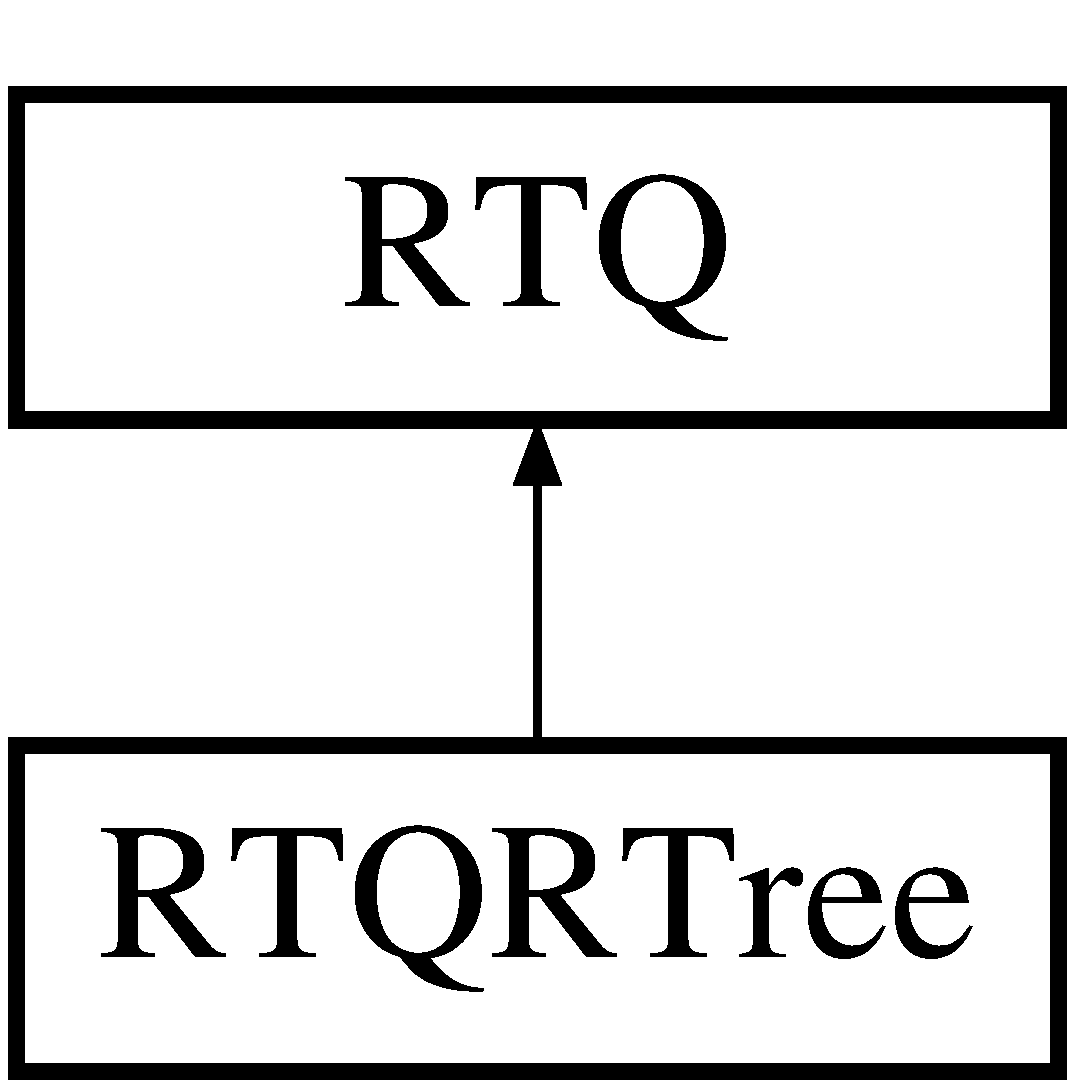
\includegraphics[height=2.000000cm]{class_r_t_q}
\end{center}
\end{figure}
\subsection*{\-Public \-Member \-Functions}
\begin{DoxyCompactItemize}
\item 
virtual void \hyperlink{class_r_t_q_a6735bb4974ca680b5dc2367b98dc11eb}{build} (const vector$<$ pair$<$ \-Index, \-Index $>$ $>$ \&\-Q, const vector$<$ pair$<$ \-Index, \-Index $>$ $>$ \&\-V)=0
\begin{DoxyCompactList}\small\item\em \-Builds structure \hyperlink{class_r_t_q}{\-R\-T\-Q}. \end{DoxyCompactList}\item 
\hypertarget{class_r_t_q_a99dfe8340d96d3d78c9df1f5eed74471}{virtual vector$<$ pair$<$ \-Index, \*
\-Index $>$ $>$ \hyperlink{class_r_t_q_a99dfe8340d96d3d78c9df1f5eed74471}{query} (\-Index x\-Min, \-Index x\-Max, \-Index y\-Min, \-Index y\-Max)=0}\label{class_r_t_q_a99dfe8340d96d3d78c9df1f5eed74471}

\begin{DoxyCompactList}\small\item\em \-Returns values (v,k) from \-V of all points (x,y) from \-Q such that (x\-Min $<$= x $<$= x\-Max) and (y\-Min $<$= y $<$= y\-Max). \end{DoxyCompactList}\end{DoxyCompactItemize}


\subsection{\-Detailed \-Description}
\-Interface for \hyperlink{class_r_t_q}{\-R\-T\-Q} geometric structure. 

\hyperlink{class_r_t_q}{\-R\-T\-Q} is geometric data structure that contains set of 2\-D-\/grid points \-Q and set of values (v, k) where each value (v,k) corresponds to one point from \-Q. \-Supports orthogonal range queries in \-Q and returns corresponding data (v,k) for each matched point. 

\subsection{\-Member \-Function \-Documentation}
\hypertarget{class_r_t_q_a6735bb4974ca680b5dc2367b98dc11eb}{\index{\-R\-T\-Q@{\-R\-T\-Q}!build@{build}}
\index{build@{build}!RTQ@{\-R\-T\-Q}}
\subsubsection[{build}]{\setlength{\rightskip}{0pt plus 5cm}virtual void {\bf \-R\-T\-Q\-::build} (
\begin{DoxyParamCaption}
\item[{const vector$<$ pair$<$ \-Index, \-Index $>$ $>$ \&}]{\-Q, }
\item[{const vector$<$ pair$<$ \-Index, \-Index $>$ $>$ \&}]{\-V}
\end{DoxyParamCaption}
)\hspace{0.3cm}{\ttfamily  \mbox{[}pure virtual\mbox{]}}}}\label{class_r_t_q_a6735bb4974ca680b5dc2367b98dc11eb}


\-Builds structure \hyperlink{class_r_t_q}{\-R\-T\-Q}. 


\begin{DoxyParams}{\-Parameters}
{\em \-Q} & \-Set of points \\
\hline
{\em \-V} & \-Set of values, \-V\mbox{[}i\mbox{]} corresponds(belongs) to \-Q\mbox{[}i\mbox{]} \\
\hline
\end{DoxyParams}


\-Implemented in \hyperlink{class_r_t_q_r_tree_a5ad156987c9c875f0c87d2030989847d}{\-R\-T\-Q\-R\-Tree}.



\-The documentation for this class was generated from the following file\-:\begin{DoxyCompactItemize}
\item 
\-R\-T\-Q.\-hpp\end{DoxyCompactItemize}

\hypertarget{class_r_t_q_r_tree}{\section{\-R\-T\-Q\-R\-Tree \-Class \-Reference}
\label{class_r_t_q_r_tree}\index{\-R\-T\-Q\-R\-Tree@{\-R\-T\-Q\-R\-Tree}}
}


\-Implementation of \hyperlink{class_r_t_q}{\-R\-T\-Q} using \-R\-Tree\-Template.  




{\ttfamily \#include $<$\-R\-T\-Q\-R\-Tree.\-hpp$>$}

\-Inheritance diagram for \-R\-T\-Q\-R\-Tree\-:\begin{figure}[H]
\begin{center}
\leavevmode
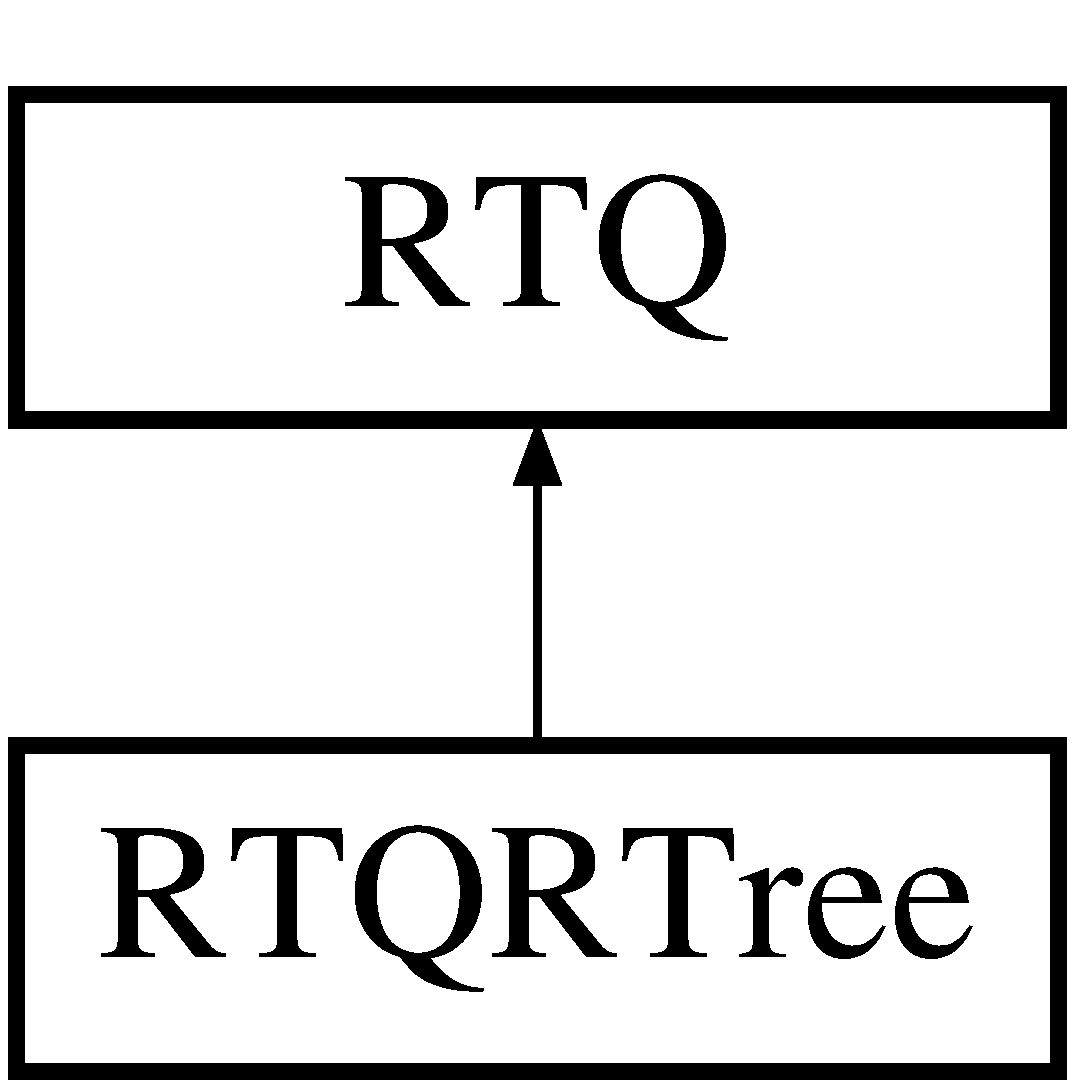
\includegraphics[height=2.000000cm]{class_r_t_q_r_tree}
\end{center}
\end{figure}
\subsection*{\-Public \-Member \-Functions}
\begin{DoxyCompactItemize}
\item 
\hypertarget{class_r_t_q_r_tree_a5ad156987c9c875f0c87d2030989847d}{void \hyperlink{class_r_t_q_r_tree_a5ad156987c9c875f0c87d2030989847d}{build} (const vector$<$ pair$<$ \-Index, \-Index $>$ $>$ \&\-Q, const vector$<$ pair$<$ \-Index, \-Index $>$ $>$ \&\-V)}\label{class_r_t_q_r_tree_a5ad156987c9c875f0c87d2030989847d}

\begin{DoxyCompactList}\small\item\em \end{DoxyCompactList}\item 
\hypertarget{class_r_t_q_r_tree_a00f5a820e471e70c911c3402ac270ea5}{vector$<$ pair$<$ \-Index, \-Index $>$ $>$ \hyperlink{class_r_t_q_r_tree_a00f5a820e471e70c911c3402ac270ea5}{query} (\-Index x\-Min, \-Index x\-Max, \-Index y\-Min, \-Index y\-Max)}\label{class_r_t_q_r_tree_a00f5a820e471e70c911c3402ac270ea5}

\begin{DoxyCompactList}\small\item\em \-Time complexity\-: \-Ideal would be \-O(log(log $|$\-Q$|$) + q), but this implementation is (log($|$\-Q$|$) + q), where q is the number of points retrieved by a query. \end{DoxyCompactList}\end{DoxyCompactItemize}


\subsection{\-Detailed \-Description}
\-Implementation of \hyperlink{class_r_t_q}{\-R\-T\-Q} using \-R\-Tree\-Template. 

// \href{https://github.com/nushoin/RTree}{\tt https\-://github.\-com/nushoin/\-R\-Tree} \-Memory usage\-: \-O($|$\-Q$|$ $\ast$ log($|$\-Q$|$)). 

\-The documentation for this class was generated from the following files\-:\begin{DoxyCompactItemize}
\item 
\-R\-T\-Q\-R\-Tree.\-hpp\item 
\-R\-T\-Q\-R\-Tree.\-cpp\end{DoxyCompactItemize}

\hypertarget{class_r_tree}{\section{\-R\-Tree$<$ \-D\-A\-T\-A\-T\-Y\-P\-E, \-E\-L\-E\-M\-T\-Y\-P\-E, \-N\-U\-M\-D\-I\-M\-S, \-E\-L\-E\-M\-T\-Y\-P\-E\-R\-E\-A\-L, \-T\-M\-A\-X\-N\-O\-D\-E\-S, \-T\-M\-I\-N\-N\-O\-D\-E\-S $>$ \-Class \-Template \-Reference}
\label{class_r_tree}\index{\-R\-Tree$<$ D\-A\-T\-A\-T\-Y\-P\-E, E\-L\-E\-M\-T\-Y\-P\-E, N\-U\-M\-D\-I\-M\-S, E\-L\-E\-M\-T\-Y\-P\-E\-R\-E\-A\-L, T\-M\-A\-X\-N\-O\-D\-E\-S, T\-M\-I\-N\-N\-O\-D\-E\-S $>$@{\-R\-Tree$<$ D\-A\-T\-A\-T\-Y\-P\-E, E\-L\-E\-M\-T\-Y\-P\-E, N\-U\-M\-D\-I\-M\-S, E\-L\-E\-M\-T\-Y\-P\-E\-R\-E\-A\-L, T\-M\-A\-X\-N\-O\-D\-E\-S, T\-M\-I\-N\-N\-O\-D\-E\-S $>$}}
}


\-Implementation of \hyperlink{class_r_tree}{\-R\-Tree}, a multidimensional bounding rectangle tree.  




{\ttfamily \#include $<$\-R\-Tree.\-hpp$>$}

\subsection*{\-Classes}
\begin{DoxyCompactItemize}
\item 
struct \hyperlink{struct_r_tree_1_1_branch}{\-Branch}
\begin{DoxyCompactList}\small\item\em \-May be data or may be another subtree \-The parents level determines this. \end{DoxyCompactList}\item 
class \hyperlink{class_r_tree_1_1_iterator}{\-Iterator}
\begin{DoxyCompactList}\small\item\em \hyperlink{class_r_tree_1_1_iterator}{\-Iterator} is not remove safe. \end{DoxyCompactList}\item 
struct \hyperlink{struct_r_tree_1_1_list_node}{\-List\-Node}
\begin{DoxyCompactList}\small\item\em \-A link list of nodes for reinsertion after a delete operation. \end{DoxyCompactList}\item 
struct \hyperlink{struct_r_tree_1_1_node}{\-Node}
\begin{DoxyCompactList}\small\item\em \hyperlink{struct_r_tree_1_1_node}{\-Node} for each branch level. \end{DoxyCompactList}\item 
struct \hyperlink{struct_r_tree_1_1_partition_vars}{\-Partition\-Vars}
\begin{DoxyCompactList}\small\item\em \-Variables for finding a split partition. \end{DoxyCompactList}\item 
struct \hyperlink{struct_r_tree_1_1_rect}{\-Rect}
\begin{DoxyCompactList}\small\item\em \-Minimal bounding rectangle (n-\/dimensional) \end{DoxyCompactList}\end{DoxyCompactItemize}
\subsection*{\-Public \-Types}
\begin{DoxyCompactItemize}
\item 
enum \{ \hyperlink{class_r_tree_afaccb2e611f17ff46b623771ad7043d7ac05afe446df73fa67991e5199453a37f}{\-M\-A\-X\-N\-O\-D\-E\-S} =  \-T\-M\-A\-X\-N\-O\-D\-E\-S, 
\hyperlink{class_r_tree_afaccb2e611f17ff46b623771ad7043d7a3be3d8c82fd5bfbd5e5a496e9877d71a}{\-M\-I\-N\-N\-O\-D\-E\-S} =  \-T\-M\-I\-N\-N\-O\-D\-E\-S
 \}
\end{DoxyCompactItemize}
\subsection*{\-Public \-Member \-Functions}
\begin{DoxyCompactItemize}
\item 
void \hyperlink{class_r_tree_a98d1f0a325921db826b2a2d5a407c9be}{\-Insert} (const \-E\-L\-E\-M\-T\-Y\-P\-E a\-\_\-min\mbox{[}\-N\-U\-M\-D\-I\-M\-S\mbox{]}, const \-E\-L\-E\-M\-T\-Y\-P\-E a\-\_\-max\mbox{[}\-N\-U\-M\-D\-I\-M\-S\mbox{]}, const \-D\-A\-T\-A\-T\-Y\-P\-E \&a\-\_\-data\-Id)
\begin{DoxyCompactList}\small\item\em \-Insert entry. \end{DoxyCompactList}\item 
void \hyperlink{class_r_tree_a1b4b6b4c73bc47029ba696c49265c043}{\-Remove} (const \-E\-L\-E\-M\-T\-Y\-P\-E a\-\_\-min\mbox{[}\-N\-U\-M\-D\-I\-M\-S\mbox{]}, const \-E\-L\-E\-M\-T\-Y\-P\-E a\-\_\-max\mbox{[}\-N\-U\-M\-D\-I\-M\-S\mbox{]}, const \-D\-A\-T\-A\-T\-Y\-P\-E \&a\-\_\-data\-Id)
\begin{DoxyCompactList}\small\item\em \-Remove entry. \end{DoxyCompactList}\item 
int \hyperlink{class_r_tree_ae9bce2b305f6e84f57f05dcab3f19156}{\-Search} (const \-E\-L\-E\-M\-T\-Y\-P\-E a\-\_\-min\mbox{[}\-N\-U\-M\-D\-I\-M\-S\mbox{]}, const \-E\-L\-E\-M\-T\-Y\-P\-E a\-\_\-max\mbox{[}\-N\-U\-M\-D\-I\-M\-S\mbox{]}, bool a\-\_\-result\-Callback(\-D\-A\-T\-A\-T\-Y\-P\-E a\-\_\-data, void $\ast$a\-\_\-context), void $\ast$a\-\_\-context)
\begin{DoxyCompactList}\small\item\em \-Find all within search rectangle. \end{DoxyCompactList}\item 
\hypertarget{class_r_tree_a396f1031eb2c8224715741fd0b77349d}{void \hyperlink{class_r_tree_a396f1031eb2c8224715741fd0b77349d}{\-Remove\-All} ()}\label{class_r_tree_a396f1031eb2c8224715741fd0b77349d}

\begin{DoxyCompactList}\small\item\em \-Remove all entries from tree. \end{DoxyCompactList}\item 
\hypertarget{class_r_tree_a813cdf63ce3e3e255821d9ba4bc9e7df}{int \hyperlink{class_r_tree_a813cdf63ce3e3e255821d9ba4bc9e7df}{\-Count} ()}\label{class_r_tree_a813cdf63ce3e3e255821d9ba4bc9e7df}

\begin{DoxyCompactList}\small\item\em \-Count the data elements in this container. \-This is slow as no internal counter is maintained. \end{DoxyCompactList}\item 
\hypertarget{class_r_tree_adbd1f87715d22ed75b2b8be738583fc2}{bool \hyperlink{class_r_tree_adbd1f87715d22ed75b2b8be738583fc2}{\-Load} (const char $\ast$a\-\_\-file\-Name)}\label{class_r_tree_adbd1f87715d22ed75b2b8be738583fc2}

\begin{DoxyCompactList}\small\item\em \-Load tree contents from file. \end{DoxyCompactList}\item 
\hypertarget{class_r_tree_ad02dc25a34d9b5b291c8ff3f1b002b09}{bool \hyperlink{class_r_tree_ad02dc25a34d9b5b291c8ff3f1b002b09}{\-Load} (\hyperlink{class_r_t_file_stream}{\-R\-T\-File\-Stream} \&a\-\_\-stream)}\label{class_r_tree_ad02dc25a34d9b5b291c8ff3f1b002b09}

\begin{DoxyCompactList}\small\item\em \-Load tree contents from stream. \end{DoxyCompactList}\item 
\hypertarget{class_r_tree_a6817692e1e8e416843be1ea628f7a074}{bool \hyperlink{class_r_tree_a6817692e1e8e416843be1ea628f7a074}{\-Save} (const char $\ast$a\-\_\-file\-Name)}\label{class_r_tree_a6817692e1e8e416843be1ea628f7a074}

\begin{DoxyCompactList}\small\item\em \-Save tree contents to file. \end{DoxyCompactList}\item 
\hypertarget{class_r_tree_a7066ea753180537a3a870c84e4fcefce}{bool \hyperlink{class_r_tree_a7066ea753180537a3a870c84e4fcefce}{\-Save} (\hyperlink{class_r_t_file_stream}{\-R\-T\-File\-Stream} \&a\-\_\-stream)}\label{class_r_tree_a7066ea753180537a3a870c84e4fcefce}

\begin{DoxyCompactList}\small\item\em \-Save tree contents to stream. \end{DoxyCompactList}\item 
\hypertarget{class_r_tree_acbcbd987b4f6549cd53e373e01b74efa}{void \hyperlink{class_r_tree_acbcbd987b4f6549cd53e373e01b74efa}{\-Get\-First} (\hyperlink{class_r_tree_1_1_iterator}{\-Iterator} \&a\-\_\-it)}\label{class_r_tree_acbcbd987b4f6549cd53e373e01b74efa}

\begin{DoxyCompactList}\small\item\em \-Get 'first' for iteration. \end{DoxyCompactList}\item 
\hypertarget{class_r_tree_a41da97d27b44e7d7e852150ced23a610}{void \hyperlink{class_r_tree_a41da97d27b44e7d7e852150ced23a610}{\-Get\-Next} (\hyperlink{class_r_tree_1_1_iterator}{\-Iterator} \&a\-\_\-it)}\label{class_r_tree_a41da97d27b44e7d7e852150ced23a610}

\begin{DoxyCompactList}\small\item\em \-Get \-Next for iteration. \end{DoxyCompactList}\item 
\hypertarget{class_r_tree_a8b8c51698e5b8df1e715650a43aad7f4}{bool \hyperlink{class_r_tree_a8b8c51698e5b8df1e715650a43aad7f4}{\-Is\-Null} (\hyperlink{class_r_tree_1_1_iterator}{\-Iterator} \&a\-\_\-it)}\label{class_r_tree_a8b8c51698e5b8df1e715650a43aad7f4}

\begin{DoxyCompactList}\small\item\em \-Is iterator \-N\-U\-L\-L, or at end? \end{DoxyCompactList}\item 
\hypertarget{class_r_tree_aab228fbd816b5e5c93666c37b47635f3}{\-D\-A\-T\-A\-T\-Y\-P\-E \& \hyperlink{class_r_tree_aab228fbd816b5e5c93666c37b47635f3}{\-Get\-At} (\hyperlink{class_r_tree_1_1_iterator}{\-Iterator} \&a\-\_\-it)}\label{class_r_tree_aab228fbd816b5e5c93666c37b47635f3}

\begin{DoxyCompactList}\small\item\em \-Get object at iterator position. \end{DoxyCompactList}\end{DoxyCompactItemize}
\subsection*{\-Protected \-Member \-Functions}
\begin{DoxyCompactItemize}
\item 
\hypertarget{class_r_tree_af118b3fc992c88a61fb2e1ebc0c96fc9}{\hyperlink{struct_r_tree_1_1_node}{\-Node} $\ast$ {\bfseries \-Alloc\-Node} ()}\label{class_r_tree_af118b3fc992c88a61fb2e1ebc0c96fc9}

\item 
\hypertarget{class_r_tree_a6b5438d9cb74dbfc63f3bfff275f506b}{void {\bfseries \-Free\-Node} (\hyperlink{struct_r_tree_1_1_node}{\-Node} $\ast$a\-\_\-node)}\label{class_r_tree_a6b5438d9cb74dbfc63f3bfff275f506b}

\item 
\hypertarget{class_r_tree_aa24d93770aaa1042136daeabfdb8de3e}{void {\bfseries \-Init\-Node} (\hyperlink{struct_r_tree_1_1_node}{\-Node} $\ast$a\-\_\-node)}\label{class_r_tree_aa24d93770aaa1042136daeabfdb8de3e}

\item 
\hypertarget{class_r_tree_aa065e71784e5cac81acd16c07c6abe5e}{void {\bfseries \-Init\-Rect} (\hyperlink{struct_r_tree_1_1_rect}{\-Rect} $\ast$a\-\_\-rect)}\label{class_r_tree_aa065e71784e5cac81acd16c07c6abe5e}

\item 
\hypertarget{class_r_tree_a534acb51413cea9ba14cdf6de955a063}{bool {\bfseries \-Insert\-Rect\-Rec} (\hyperlink{struct_r_tree_1_1_rect}{\-Rect} $\ast$a\-\_\-rect, const \-D\-A\-T\-A\-T\-Y\-P\-E \&a\-\_\-id, \hyperlink{struct_r_tree_1_1_node}{\-Node} $\ast$a\-\_\-node, \hyperlink{struct_r_tree_1_1_node}{\-Node} $\ast$$\ast$a\-\_\-new\-Node, int a\-\_\-level)}\label{class_r_tree_a534acb51413cea9ba14cdf6de955a063}

\item 
\hypertarget{class_r_tree_a0539c68da4aec2165a14ee2c93fab028}{bool {\bfseries \-Insert\-Rect} (\hyperlink{struct_r_tree_1_1_rect}{\-Rect} $\ast$a\-\_\-rect, const \-D\-A\-T\-A\-T\-Y\-P\-E \&a\-\_\-id, \hyperlink{struct_r_tree_1_1_node}{\-Node} $\ast$$\ast$a\-\_\-root, int a\-\_\-level)}\label{class_r_tree_a0539c68da4aec2165a14ee2c93fab028}

\item 
\hypertarget{class_r_tree_a19dc96034d7a3230ba877953247457e1}{\hyperlink{struct_r_tree_1_1_rect}{\-Rect} {\bfseries \-Node\-Cover} (\hyperlink{struct_r_tree_1_1_node}{\-Node} $\ast$a\-\_\-node)}\label{class_r_tree_a19dc96034d7a3230ba877953247457e1}

\item 
\hypertarget{class_r_tree_af73c482c9a170955c874399a78b8091e}{bool {\bfseries \-Add\-Branch} (\hyperlink{struct_r_tree_1_1_branch}{\-Branch} $\ast$a\-\_\-branch, \hyperlink{struct_r_tree_1_1_node}{\-Node} $\ast$a\-\_\-node, \hyperlink{struct_r_tree_1_1_node}{\-Node} $\ast$$\ast$a\-\_\-new\-Node)}\label{class_r_tree_af73c482c9a170955c874399a78b8091e}

\item 
\hypertarget{class_r_tree_adcdcac926b2de35cc1f4f07e02b70bf6}{void {\bfseries \-Disconnect\-Branch} (\hyperlink{struct_r_tree_1_1_node}{\-Node} $\ast$a\-\_\-node, int a\-\_\-index)}\label{class_r_tree_adcdcac926b2de35cc1f4f07e02b70bf6}

\item 
\hypertarget{class_r_tree_a7c70c0761eb2c0e77db4cf846603d624}{int {\bfseries \-Pick\-Branch} (\hyperlink{struct_r_tree_1_1_rect}{\-Rect} $\ast$a\-\_\-rect, \hyperlink{struct_r_tree_1_1_node}{\-Node} $\ast$a\-\_\-node)}\label{class_r_tree_a7c70c0761eb2c0e77db4cf846603d624}

\item 
\hypertarget{class_r_tree_a90c2c0887fc456d2e9c7953e657958a7}{\hyperlink{struct_r_tree_1_1_rect}{\-Rect} {\bfseries \-Combine\-Rect} (\hyperlink{struct_r_tree_1_1_rect}{\-Rect} $\ast$a\-\_\-rect\-A, \hyperlink{struct_r_tree_1_1_rect}{\-Rect} $\ast$a\-\_\-rect\-B)}\label{class_r_tree_a90c2c0887fc456d2e9c7953e657958a7}

\item 
\hypertarget{class_r_tree_a38e60b3f2e970394492c8c6955375bec}{void {\bfseries \-Split\-Node} (\hyperlink{struct_r_tree_1_1_node}{\-Node} $\ast$a\-\_\-node, \hyperlink{struct_r_tree_1_1_branch}{\-Branch} $\ast$a\-\_\-branch, \hyperlink{struct_r_tree_1_1_node}{\-Node} $\ast$$\ast$a\-\_\-new\-Node)}\label{class_r_tree_a38e60b3f2e970394492c8c6955375bec}

\item 
\hypertarget{class_r_tree_a7958e17fc046e5d648d8e23ffc82e849}{\-E\-L\-E\-M\-T\-Y\-P\-E\-R\-E\-A\-L {\bfseries \-Rect\-Spherical\-Volume} (\hyperlink{struct_r_tree_1_1_rect}{\-Rect} $\ast$a\-\_\-rect)}\label{class_r_tree_a7958e17fc046e5d648d8e23ffc82e849}

\item 
\hypertarget{class_r_tree_af9f63fef551a4c3a42cd915618a9917a}{\-E\-L\-E\-M\-T\-Y\-P\-E\-R\-E\-A\-L {\bfseries \-Rect\-Volume} (\hyperlink{struct_r_tree_1_1_rect}{\-Rect} $\ast$a\-\_\-rect)}\label{class_r_tree_af9f63fef551a4c3a42cd915618a9917a}

\item 
\hypertarget{class_r_tree_a224ba0af4dcb435dbb016327307d664b}{\-E\-L\-E\-M\-T\-Y\-P\-E\-R\-E\-A\-L {\bfseries \-Calc\-Rect\-Volume} (\hyperlink{struct_r_tree_1_1_rect}{\-Rect} $\ast$a\-\_\-rect)}\label{class_r_tree_a224ba0af4dcb435dbb016327307d664b}

\item 
\hypertarget{class_r_tree_a2b9d627796433f3b0254a541c19ed450}{void {\bfseries \-Get\-Branches} (\hyperlink{struct_r_tree_1_1_node}{\-Node} $\ast$a\-\_\-node, \hyperlink{struct_r_tree_1_1_branch}{\-Branch} $\ast$a\-\_\-branch, \hyperlink{struct_r_tree_1_1_partition_vars}{\-Partition\-Vars} $\ast$a\-\_\-par\-Vars)}\label{class_r_tree_a2b9d627796433f3b0254a541c19ed450}

\item 
\hypertarget{class_r_tree_a282f6ef6b93f714d8a8eca3c4d587cbd}{void {\bfseries \-Choose\-Partition} (\hyperlink{struct_r_tree_1_1_partition_vars}{\-Partition\-Vars} $\ast$a\-\_\-par\-Vars, int a\-\_\-min\-Fill)}\label{class_r_tree_a282f6ef6b93f714d8a8eca3c4d587cbd}

\item 
\hypertarget{class_r_tree_a88e9eef4ad30d4dee0c783df5e6840a0}{void {\bfseries \-Load\-Nodes} (\hyperlink{struct_r_tree_1_1_node}{\-Node} $\ast$a\-\_\-node\-A, \hyperlink{struct_r_tree_1_1_node}{\-Node} $\ast$a\-\_\-node\-B, \hyperlink{struct_r_tree_1_1_partition_vars}{\-Partition\-Vars} $\ast$a\-\_\-par\-Vars)}\label{class_r_tree_a88e9eef4ad30d4dee0c783df5e6840a0}

\item 
\hypertarget{class_r_tree_aac207d4389fcca1aa0b72361d84117ec}{void {\bfseries \-Init\-Par\-Vars} (\hyperlink{struct_r_tree_1_1_partition_vars}{\-Partition\-Vars} $\ast$a\-\_\-par\-Vars, int a\-\_\-max\-Rects, int a\-\_\-min\-Fill)}\label{class_r_tree_aac207d4389fcca1aa0b72361d84117ec}

\item 
\hypertarget{class_r_tree_af4232dd5fd978fcce12ce32f9df20f58}{void {\bfseries \-Pick\-Seeds} (\hyperlink{struct_r_tree_1_1_partition_vars}{\-Partition\-Vars} $\ast$a\-\_\-par\-Vars)}\label{class_r_tree_af4232dd5fd978fcce12ce32f9df20f58}

\item 
\hypertarget{class_r_tree_a5da8614a152145988f010a0b7ff9cb4d}{void {\bfseries \-Classify} (int a\-\_\-index, int a\-\_\-group, \hyperlink{struct_r_tree_1_1_partition_vars}{\-Partition\-Vars} $\ast$a\-\_\-par\-Vars)}\label{class_r_tree_a5da8614a152145988f010a0b7ff9cb4d}

\item 
\hypertarget{class_r_tree_a64a1092e85775014ce01e1bb6bc8a938}{bool {\bfseries \-Remove\-Rect} (\hyperlink{struct_r_tree_1_1_rect}{\-Rect} $\ast$a\-\_\-rect, const \-D\-A\-T\-A\-T\-Y\-P\-E \&a\-\_\-id, \hyperlink{struct_r_tree_1_1_node}{\-Node} $\ast$$\ast$a\-\_\-root)}\label{class_r_tree_a64a1092e85775014ce01e1bb6bc8a938}

\item 
\hypertarget{class_r_tree_a519d3084a57b45ed4e4167b382bc977e}{bool {\bfseries \-Remove\-Rect\-Rec} (\hyperlink{struct_r_tree_1_1_rect}{\-Rect} $\ast$a\-\_\-rect, const \-D\-A\-T\-A\-T\-Y\-P\-E \&a\-\_\-id, \hyperlink{struct_r_tree_1_1_node}{\-Node} $\ast$a\-\_\-node, \hyperlink{struct_r_tree_1_1_list_node}{\-List\-Node} $\ast$$\ast$a\-\_\-list\-Node)}\label{class_r_tree_a519d3084a57b45ed4e4167b382bc977e}

\item 
\hypertarget{class_r_tree_aa688a31e4de0090985045cfabfa42d2d}{\hyperlink{struct_r_tree_1_1_list_node}{\-List\-Node} $\ast$ {\bfseries \-Alloc\-List\-Node} ()}\label{class_r_tree_aa688a31e4de0090985045cfabfa42d2d}

\item 
\hypertarget{class_r_tree_a0c92660832f03d899608d73b994e95a5}{void {\bfseries \-Free\-List\-Node} (\hyperlink{struct_r_tree_1_1_list_node}{\-List\-Node} $\ast$a\-\_\-list\-Node)}\label{class_r_tree_a0c92660832f03d899608d73b994e95a5}

\item 
\hypertarget{class_r_tree_aa5b369536a94aa8ad9ec3b4f8f68302c}{bool {\bfseries \-Overlap} (\hyperlink{struct_r_tree_1_1_rect}{\-Rect} $\ast$a\-\_\-rect\-A, \hyperlink{struct_r_tree_1_1_rect}{\-Rect} $\ast$a\-\_\-rect\-B)}\label{class_r_tree_aa5b369536a94aa8ad9ec3b4f8f68302c}

\item 
\hypertarget{class_r_tree_a5d2b072588eae9e9058224942ae0294f}{void {\bfseries \-Re\-Insert} (\hyperlink{struct_r_tree_1_1_node}{\-Node} $\ast$a\-\_\-node, \hyperlink{struct_r_tree_1_1_list_node}{\-List\-Node} $\ast$$\ast$a\-\_\-list\-Node)}\label{class_r_tree_a5d2b072588eae9e9058224942ae0294f}

\item 
\hypertarget{class_r_tree_af2baaed34f4e0cf20597074ebfb77ac4}{bool {\bfseries \-Search} (\hyperlink{struct_r_tree_1_1_node}{\-Node} $\ast$a\-\_\-node, \hyperlink{struct_r_tree_1_1_rect}{\-Rect} $\ast$a\-\_\-rect, int \&a\-\_\-found\-Count, bool a\-\_\-result\-Callback(\-D\-A\-T\-A\-T\-Y\-P\-E a\-\_\-data, void $\ast$a\-\_\-context), void $\ast$a\-\_\-context)}\label{class_r_tree_af2baaed34f4e0cf20597074ebfb77ac4}

\item 
\hypertarget{class_r_tree_a5045d833566114335162fda10d58081d}{void {\bfseries \-Remove\-All\-Rec} (\hyperlink{struct_r_tree_1_1_node}{\-Node} $\ast$a\-\_\-node)}\label{class_r_tree_a5045d833566114335162fda10d58081d}

\item 
\hypertarget{class_r_tree_a2508b9d85f5b5f553b313356c05c6e0c}{void {\bfseries \-Reset} ()}\label{class_r_tree_a2508b9d85f5b5f553b313356c05c6e0c}

\item 
\hypertarget{class_r_tree_a22345d494c1d6bf907444f17802bd864}{void {\bfseries \-Count\-Rec} (\hyperlink{struct_r_tree_1_1_node}{\-Node} $\ast$a\-\_\-node, int \&a\-\_\-count)}\label{class_r_tree_a22345d494c1d6bf907444f17802bd864}

\item 
\hypertarget{class_r_tree_a53a8af8a04a9a4a9eb93a6a0792fea95}{bool {\bfseries \-Save\-Rec} (\hyperlink{struct_r_tree_1_1_node}{\-Node} $\ast$a\-\_\-node, \hyperlink{class_r_t_file_stream}{\-R\-T\-File\-Stream} \&a\-\_\-stream)}\label{class_r_tree_a53a8af8a04a9a4a9eb93a6a0792fea95}

\item 
\hypertarget{class_r_tree_aa432ad1d5dfc151c1f8eac388af41968}{bool {\bfseries \-Load\-Rec} (\hyperlink{struct_r_tree_1_1_node}{\-Node} $\ast$a\-\_\-node, \hyperlink{class_r_t_file_stream}{\-R\-T\-File\-Stream} \&a\-\_\-stream)}\label{class_r_tree_aa432ad1d5dfc151c1f8eac388af41968}

\end{DoxyCompactItemize}
\subsection*{\-Protected \-Attributes}
\begin{DoxyCompactItemize}
\item 
\hypertarget{class_r_tree_a5028f4e28918519bc70cb1f615316582}{\hyperlink{struct_r_tree_1_1_node}{\-Node} $\ast$ \hyperlink{class_r_tree_a5028f4e28918519bc70cb1f615316582}{m\-\_\-root}}\label{class_r_tree_a5028f4e28918519bc70cb1f615316582}

\begin{DoxyCompactList}\small\item\em \-Root of tree. \end{DoxyCompactList}\item 
\hypertarget{class_r_tree_af26d4beb8ce3a381ee75eabeec4727e3}{\-E\-L\-E\-M\-T\-Y\-P\-E\-R\-E\-A\-L \hyperlink{class_r_tree_af26d4beb8ce3a381ee75eabeec4727e3}{m\-\_\-unit\-Sphere\-Volume}}\label{class_r_tree_af26d4beb8ce3a381ee75eabeec4727e3}

\begin{DoxyCompactList}\small\item\em \-Unit sphere constant for required number of dimensions. \end{DoxyCompactList}\end{DoxyCompactItemize}


\subsection{\-Detailed \-Description}
\subsubsection*{template$<$class \-D\-A\-T\-A\-T\-Y\-P\-E, class \-E\-L\-E\-M\-T\-Y\-P\-E, int \-N\-U\-M\-D\-I\-M\-S, class \-E\-L\-E\-M\-T\-Y\-P\-E\-R\-E\-A\-L = \-E\-L\-E\-M\-T\-Y\-P\-E, int \-T\-M\-A\-X\-N\-O\-D\-E\-S = 8, int \-T\-M\-I\-N\-N\-O\-D\-E\-S = \-T\-M\-A\-X\-N\-O\-D\-E\-S / 2$>$class R\-Tree$<$ D\-A\-T\-A\-T\-Y\-P\-E, E\-L\-E\-M\-T\-Y\-P\-E, N\-U\-M\-D\-I\-M\-S, E\-L\-E\-M\-T\-Y\-P\-E\-R\-E\-A\-L, T\-M\-A\-X\-N\-O\-D\-E\-S, T\-M\-I\-N\-N\-O\-D\-E\-S $>$}

\-Implementation of \hyperlink{class_r_tree}{\-R\-Tree}, a multidimensional bounding rectangle tree. 

\-Example usage\-: \-For a 3-\/dimensional tree use \-R\-Tree$<$\-Object$\ast$, float, 3$>$ my\-Tree;

\-This modified, templated \-C++ version by \-Greg \-Douglas at \-Auran (\href{http://www.auran.com}{\tt http\-://www.\-auran.\-com})

\-D\-A\-T\-A\-T\-Y\-P\-E \-Referenced data, should be int, void$\ast$, obj$\ast$ etc. no larger than sizeof$<$void$\ast$$>$ and simple type \-E\-L\-E\-M\-T\-Y\-P\-E \-Type of element such as int or float \-N\-U\-M\-D\-I\-M\-S \-Number of dimensions such as 2 or 3 \-E\-L\-E\-M\-T\-Y\-P\-E\-R\-E\-A\-L \-Type of element that allows fractional and large values such as float or double, for use in volume calcs

\-N\-O\-T\-E\-S\-: \-Inserting and removing data requires the knowledge of its constant \-Minimal \-Bounding \-Rectangle. \-This version uses new/delete for nodes, \-I recommend using a fixed size allocator for efficiency. \-Instead of using a callback function for returned results, \-I recommend and efficient pre-\/sized, grow-\/only memory array similar to \-M\-F\-C \-C\-Array or \-S\-T\-L \-Vector for returning search query result. 

\subsection{\-Member \-Enumeration \-Documentation}
\hypertarget{class_r_tree_afaccb2e611f17ff46b623771ad7043d7}{\subsubsection[{anonymous enum}]{\setlength{\rightskip}{0pt plus 5cm}template$<$class \-D\-A\-T\-A\-T\-Y\-P\-E, class \-E\-L\-E\-M\-T\-Y\-P\-E, int \-N\-U\-M\-D\-I\-M\-S, class \-E\-L\-E\-M\-T\-Y\-P\-E\-R\-E\-A\-L = \-E\-L\-E\-M\-T\-Y\-P\-E, int \-T\-M\-A\-X\-N\-O\-D\-E\-S = 8, int \-T\-M\-I\-N\-N\-O\-D\-E\-S = \-T\-M\-A\-X\-N\-O\-D\-E\-S / 2$>$ anonymous enum}}\label{class_r_tree_afaccb2e611f17ff46b623771ad7043d7}
\begin{Desc}
\item[\-Enumerator\-: ]\par
\begin{description}
\index{\-M\-A\-X\-N\-O\-D\-E\-S@{\-M\-A\-X\-N\-O\-D\-E\-S}!\-R\-Tree@{\-R\-Tree}}\index{\-R\-Tree@{\-R\-Tree}!\-M\-A\-X\-N\-O\-D\-E\-S@{\-M\-A\-X\-N\-O\-D\-E\-S}}\item[{\em 
\hypertarget{class_r_tree_afaccb2e611f17ff46b623771ad7043d7ac05afe446df73fa67991e5199453a37f}{\-M\-A\-X\-N\-O\-D\-E\-S}\label{class_r_tree_afaccb2e611f17ff46b623771ad7043d7ac05afe446df73fa67991e5199453a37f}
}]\-Max elements in node. \index{\-M\-I\-N\-N\-O\-D\-E\-S@{\-M\-I\-N\-N\-O\-D\-E\-S}!\-R\-Tree@{\-R\-Tree}}\index{\-R\-Tree@{\-R\-Tree}!\-M\-I\-N\-N\-O\-D\-E\-S@{\-M\-I\-N\-N\-O\-D\-E\-S}}\item[{\em 
\hypertarget{class_r_tree_afaccb2e611f17ff46b623771ad7043d7a3be3d8c82fd5bfbd5e5a496e9877d71a}{\-M\-I\-N\-N\-O\-D\-E\-S}\label{class_r_tree_afaccb2e611f17ff46b623771ad7043d7a3be3d8c82fd5bfbd5e5a496e9877d71a}
}]\-Min elements in node. \end{description}
\end{Desc}



\subsection{\-Member \-Function \-Documentation}
\hypertarget{class_r_tree_a98d1f0a325921db826b2a2d5a407c9be}{\index{\-R\-Tree@{\-R\-Tree}!\-Insert@{\-Insert}}
\index{\-Insert@{\-Insert}!RTree@{\-R\-Tree}}
\subsubsection[{\-Insert}]{\setlength{\rightskip}{0pt plus 5cm}template$<$class \-D\-A\-T\-A\-T\-Y\-P\-E, class \-E\-L\-E\-M\-T\-Y\-P\-E, int \-N\-U\-M\-D\-I\-M\-S, class \-E\-L\-E\-M\-T\-Y\-P\-E\-R\-E\-A\-L = \-E\-L\-E\-M\-T\-Y\-P\-E, int \-T\-M\-A\-X\-N\-O\-D\-E\-S = 8, int \-T\-M\-I\-N\-N\-O\-D\-E\-S = \-T\-M\-A\-X\-N\-O\-D\-E\-S / 2$>$ void {\bf \-R\-Tree}$<$ \-D\-A\-T\-A\-T\-Y\-P\-E, \-E\-L\-E\-M\-T\-Y\-P\-E, \-N\-U\-M\-D\-I\-M\-S, \-E\-L\-E\-M\-T\-Y\-P\-E\-R\-E\-A\-L, \-T\-M\-A\-X\-N\-O\-D\-E\-S, \-T\-M\-I\-N\-N\-O\-D\-E\-S $>$\-::{\bf \-Insert} (
\begin{DoxyParamCaption}
\item[{const \-E\-L\-E\-M\-T\-Y\-P\-E}]{a\-\_\-min\mbox{[}\-N\-U\-M\-D\-I\-M\-S\mbox{]}, }
\item[{const \-E\-L\-E\-M\-T\-Y\-P\-E}]{a\-\_\-max\mbox{[}\-N\-U\-M\-D\-I\-M\-S\mbox{]}, }
\item[{const \-D\-A\-T\-A\-T\-Y\-P\-E \&}]{a\-\_\-data\-Id}
\end{DoxyParamCaption}
)}}\label{class_r_tree_a98d1f0a325921db826b2a2d5a407c9be}


\-Insert entry. 


\begin{DoxyParams}{\-Parameters}
{\em a\-\_\-min} & \-Min of bounding rect \\
\hline
{\em a\-\_\-max} & \-Max of bounding rect \\
\hline
{\em a\-\_\-data\-Id} & \-Positive \-Id of data. \-Maybe zero, but negative numbers not allowed. \\
\hline
\end{DoxyParams}
\hypertarget{class_r_tree_a1b4b6b4c73bc47029ba696c49265c043}{\index{\-R\-Tree@{\-R\-Tree}!\-Remove@{\-Remove}}
\index{\-Remove@{\-Remove}!RTree@{\-R\-Tree}}
\subsubsection[{\-Remove}]{\setlength{\rightskip}{0pt plus 5cm}template$<$class \-D\-A\-T\-A\-T\-Y\-P\-E, class \-E\-L\-E\-M\-T\-Y\-P\-E, int \-N\-U\-M\-D\-I\-M\-S, class \-E\-L\-E\-M\-T\-Y\-P\-E\-R\-E\-A\-L = \-E\-L\-E\-M\-T\-Y\-P\-E, int \-T\-M\-A\-X\-N\-O\-D\-E\-S = 8, int \-T\-M\-I\-N\-N\-O\-D\-E\-S = \-T\-M\-A\-X\-N\-O\-D\-E\-S / 2$>$ void {\bf \-R\-Tree}$<$ \-D\-A\-T\-A\-T\-Y\-P\-E, \-E\-L\-E\-M\-T\-Y\-P\-E, \-N\-U\-M\-D\-I\-M\-S, \-E\-L\-E\-M\-T\-Y\-P\-E\-R\-E\-A\-L, \-T\-M\-A\-X\-N\-O\-D\-E\-S, \-T\-M\-I\-N\-N\-O\-D\-E\-S $>$\-::{\bf \-Remove} (
\begin{DoxyParamCaption}
\item[{const \-E\-L\-E\-M\-T\-Y\-P\-E}]{a\-\_\-min\mbox{[}\-N\-U\-M\-D\-I\-M\-S\mbox{]}, }
\item[{const \-E\-L\-E\-M\-T\-Y\-P\-E}]{a\-\_\-max\mbox{[}\-N\-U\-M\-D\-I\-M\-S\mbox{]}, }
\item[{const \-D\-A\-T\-A\-T\-Y\-P\-E \&}]{a\-\_\-data\-Id}
\end{DoxyParamCaption}
)}}\label{class_r_tree_a1b4b6b4c73bc47029ba696c49265c043}


\-Remove entry. 


\begin{DoxyParams}{\-Parameters}
{\em a\-\_\-min} & \-Min of bounding rect \\
\hline
{\em a\-\_\-max} & \-Max of bounding rect \\
\hline
{\em a\-\_\-data\-Id} & \-Positive \-Id of data. \-Maybe zero, but negative numbers not allowed. \\
\hline
\end{DoxyParams}
\hypertarget{class_r_tree_ae9bce2b305f6e84f57f05dcab3f19156}{\index{\-R\-Tree@{\-R\-Tree}!\-Search@{\-Search}}
\index{\-Search@{\-Search}!RTree@{\-R\-Tree}}
\subsubsection[{\-Search}]{\setlength{\rightskip}{0pt plus 5cm}template$<$class \-D\-A\-T\-A\-T\-Y\-P\-E, class \-E\-L\-E\-M\-T\-Y\-P\-E, int \-N\-U\-M\-D\-I\-M\-S, class \-E\-L\-E\-M\-T\-Y\-P\-E\-R\-E\-A\-L = \-E\-L\-E\-M\-T\-Y\-P\-E, int \-T\-M\-A\-X\-N\-O\-D\-E\-S = 8, int \-T\-M\-I\-N\-N\-O\-D\-E\-S = \-T\-M\-A\-X\-N\-O\-D\-E\-S / 2$>$ int {\bf \-R\-Tree}$<$ \-D\-A\-T\-A\-T\-Y\-P\-E, \-E\-L\-E\-M\-T\-Y\-P\-E, \-N\-U\-M\-D\-I\-M\-S, \-E\-L\-E\-M\-T\-Y\-P\-E\-R\-E\-A\-L, \-T\-M\-A\-X\-N\-O\-D\-E\-S, \-T\-M\-I\-N\-N\-O\-D\-E\-S $>$\-::{\bf \-Search} (
\begin{DoxyParamCaption}
\item[{const \-E\-L\-E\-M\-T\-Y\-P\-E}]{a\-\_\-min\mbox{[}\-N\-U\-M\-D\-I\-M\-S\mbox{]}, }
\item[{const \-E\-L\-E\-M\-T\-Y\-P\-E}]{a\-\_\-max\mbox{[}\-N\-U\-M\-D\-I\-M\-S\mbox{]}, }
\item[{bool }]{a\-\_\-result\-Callback\-D\-A\-T\-A\-T\-Y\-P\-E a\-\_\-data, void $\ast$a\-\_\-context, }
\item[{void $\ast$}]{a\-\_\-context}
\end{DoxyParamCaption}
)}}\label{class_r_tree_ae9bce2b305f6e84f57f05dcab3f19156}


\-Find all within search rectangle. 


\begin{DoxyParams}{\-Parameters}
{\em a\-\_\-min} & \-Min of search bounding rect \\
\hline
{\em a\-\_\-max} & \-Max of search bounding rect \\
\hline
{\em a\-\_\-search\-Result} & \-Search result array. \-Caller should set grow size. \-Function will reset, not append to array. \\
\hline
{\em a\-\_\-result\-Callback} & \-Callback function to return result. \-Callback should return 'true' to continue searching \\
\hline
{\em a\-\_\-context} & \-User context to pass as parameter to a\-\_\-result\-Callback \\
\hline
\end{DoxyParams}
\begin{DoxyReturn}{\-Returns}
\-Returns the number of entries found 
\end{DoxyReturn}


\-The documentation for this class was generated from the following file\-:\begin{DoxyCompactItemize}
\item 
\-R\-Tree.\-hpp\end{DoxyCompactItemize}

\hypertarget{class_s_a_sort}{\section{\-S\-A\-Sort \-Class \-Reference}
\label{class_s_a_sort}\index{\-S\-A\-Sort@{\-S\-A\-Sort}}
}


\-Class for comparing string suffixes.  


\subsection*{\-Public \-Member \-Functions}
\begin{DoxyCompactItemize}
\item 
\hypertarget{class_s_a_sort_ac1696867c674832f5dbf214b0a5b2ced}{{\bfseries \-S\-A\-Sort} (const string \&\-T\-\_\-)}\label{class_s_a_sort_ac1696867c674832f5dbf214b0a5b2ced}

\item 
\hypertarget{class_s_a_sort_a29a47bc0e448ad3d0cb28d8b779f11e6}{bool {\bfseries operator()} (\-Index pos1, \-Index pos2)}\label{class_s_a_sort_a29a47bc0e448ad3d0cb28d8b779f11e6}

\item 
\hypertarget{class_s_a_sort_ac1696867c674832f5dbf214b0a5b2ced}{{\bfseries \-S\-A\-Sort} (const string \&\-T\-\_\-)}\label{class_s_a_sort_ac1696867c674832f5dbf214b0a5b2ced}

\item 
\hypertarget{class_s_a_sort_a29a47bc0e448ad3d0cb28d8b779f11e6}{bool {\bfseries operator()} (\-Index pos1, \-Index pos2)}\label{class_s_a_sort_a29a47bc0e448ad3d0cb28d8b779f11e6}

\end{DoxyCompactItemize}


\subsection{\-Detailed \-Description}
\-Class for comparing string suffixes. 



\-The documentation for this class was generated from the following files\-:\begin{DoxyCompactItemize}
\item 
\-Opp/\-\_\-\-Opp\-Misc/\-Compressor\-Old/\-Compressor.\-cpp\item 
\-Opp/\-Compressor.\-cpp\end{DoxyCompactItemize}

\hypertarget{class_string_view}{\section{\-String\-View \-Class \-Reference}
\label{class_string_view}\index{\-String\-View@{\-String\-View}}
}


\hyperlink{class_string_view}{\-String\-View} is slightly changed view of another string with minimum copying involved.  




{\ttfamily \#include $<$\-String\-View.\-hpp$>$}

\subsection*{\-Public \-Member \-Functions}
\begin{DoxyCompactItemize}
\item 
\hyperlink{class_string_view_a522ccbcc302cd1abd01d680cac12ab8e}{\-String\-View} (const string \&s)
\begin{DoxyCompactList}\small\item\em \-Create a view of given string. \end{DoxyCompactList}\item 
\hyperlink{class_string_view_aa931db04bde219d3ab4352bd4e7152f1}{\-String\-View} (const string \&s, \-Index start, \-Index length)
\begin{DoxyCompactList}\small\item\em \-Create a view of given string, starting from character at position start and ending at position start+length-\/1, inclusive. \end{DoxyCompactList}\item 
\hyperlink{class_string_view_ae455a514d2b78e5f8922761aab432bce}{\-String\-View} (const string \&s, \-Index start)
\begin{DoxyCompactList}\small\item\em \-Create a view of given string, starting from character at position start and ending at position s.\-length-\/1, inclusive. \end{DoxyCompactList}\item 
void \hyperlink{class_string_view_af1005934a166e1a3939f48835a3b6533}{add\-Prefix} (const string \&prefix)
\begin{DoxyCompactList}\small\item\em \-Add prefix. \end{DoxyCompactList}\item 
void \hyperlink{class_string_view_aeb2d536a71c4c0851db6c302718d18ac}{add\-Suffix} (const string \&suffix)
\begin{DoxyCompactList}\small\item\em \-Add suffix. \end{DoxyCompactList}\item 
char \hyperlink{class_string_view_a6507eb2f61220c86a405a9df0f557fe7}{char\-At} (\-Index i) const 
\begin{DoxyCompactList}\small\item\em \-Returns char at position i. \end{DoxyCompactList}\item 
\-Index \hyperlink{class_string_view_af0857afdaefc0a484d525bfd455855d4}{get\-Length} () const 
\begin{DoxyCompactList}\small\item\em \-Returns length of preffix, viewed string and suffix together. \end{DoxyCompactList}\item 
void \hyperlink{class_string_view_a12e97255dbedce202866e0ba872a1a56}{reverse} ()
\begin{DoxyCompactList}\small\item\em \-Reverse view. \end{DoxyCompactList}\end{DoxyCompactItemize}


\subsection{\-Detailed \-Description}
\hyperlink{class_string_view}{\-String\-View} is slightly changed view of another string with minimum copying involved. 

\hyperlink{class_string_view}{\-String\-View} can not affect or change viewed string. \-We can add suffix, preffix, or limit our view to substring of viewed string. \-When making a view of another string, no copying is done. \-When adding prefix or suffix they are actually stored, so prefix and suffix should not be big. 

\subsection{\-Constructor \& \-Destructor \-Documentation}
\hypertarget{class_string_view_a522ccbcc302cd1abd01d680cac12ab8e}{\index{\-String\-View@{\-String\-View}!\-String\-View@{\-String\-View}}
\index{\-String\-View@{\-String\-View}!StringView@{\-String\-View}}
\subsubsection[{\-String\-View}]{\setlength{\rightskip}{0pt plus 5cm}{\bf \-String\-View\-::\-String\-View} (
\begin{DoxyParamCaption}
\item[{const string \&}]{s}
\end{DoxyParamCaption}
)}}\label{class_string_view_a522ccbcc302cd1abd01d680cac12ab8e}


\-Create a view of given string. 

\-Space and time complexity\-: \-O(1). \hypertarget{class_string_view_aa931db04bde219d3ab4352bd4e7152f1}{\index{\-String\-View@{\-String\-View}!\-String\-View@{\-String\-View}}
\index{\-String\-View@{\-String\-View}!StringView@{\-String\-View}}
\subsubsection[{\-String\-View}]{\setlength{\rightskip}{0pt plus 5cm}{\bf \-String\-View\-::\-String\-View} (
\begin{DoxyParamCaption}
\item[{const string \&}]{s, }
\item[{\-Index}]{start, }
\item[{\-Index}]{length}
\end{DoxyParamCaption}
)}}\label{class_string_view_aa931db04bde219d3ab4352bd4e7152f1}


\-Create a view of given string, starting from character at position start and ending at position start+length-\/1, inclusive. 

\-Space and time complexity\-: \-O(1). \hypertarget{class_string_view_ae455a514d2b78e5f8922761aab432bce}{\index{\-String\-View@{\-String\-View}!\-String\-View@{\-String\-View}}
\index{\-String\-View@{\-String\-View}!StringView@{\-String\-View}}
\subsubsection[{\-String\-View}]{\setlength{\rightskip}{0pt plus 5cm}{\bf \-String\-View\-::\-String\-View} (
\begin{DoxyParamCaption}
\item[{const string \&}]{s, }
\item[{\-Index}]{start}
\end{DoxyParamCaption}
)}}\label{class_string_view_ae455a514d2b78e5f8922761aab432bce}


\-Create a view of given string, starting from character at position start and ending at position s.\-length-\/1, inclusive. 

\-Space and time complexity\-: \-O(1). 

\subsection{\-Member \-Function \-Documentation}
\hypertarget{class_string_view_af1005934a166e1a3939f48835a3b6533}{\index{\-String\-View@{\-String\-View}!add\-Prefix@{add\-Prefix}}
\index{add\-Prefix@{add\-Prefix}!StringView@{\-String\-View}}
\subsubsection[{add\-Prefix}]{\setlength{\rightskip}{0pt plus 5cm}void {\bf \-String\-View\-::add\-Prefix} (
\begin{DoxyParamCaption}
\item[{const string \&}]{prefix}
\end{DoxyParamCaption}
)}}\label{class_string_view_af1005934a166e1a3939f48835a3b6533}


\-Add prefix. 

\-Prefix is actually copied and stored in \hyperlink{class_string_view}{\-String\-View}. \-After prefix is added, rewind is automatically called. \hypertarget{class_string_view_aeb2d536a71c4c0851db6c302718d18ac}{\index{\-String\-View@{\-String\-View}!add\-Suffix@{add\-Suffix}}
\index{add\-Suffix@{add\-Suffix}!StringView@{\-String\-View}}
\subsubsection[{add\-Suffix}]{\setlength{\rightskip}{0pt plus 5cm}void {\bf \-String\-View\-::add\-Suffix} (
\begin{DoxyParamCaption}
\item[{const string \&}]{suffix}
\end{DoxyParamCaption}
)}}\label{class_string_view_aeb2d536a71c4c0851db6c302718d18ac}


\-Add suffix. 

\-Suffix is actually copied and stored in \hyperlink{class_string_view}{\-String\-View}. \-After prefix is added, rewind is automatically called. \hypertarget{class_string_view_a6507eb2f61220c86a405a9df0f557fe7}{\index{\-String\-View@{\-String\-View}!char\-At@{char\-At}}
\index{char\-At@{char\-At}!StringView@{\-String\-View}}
\subsubsection[{char\-At}]{\setlength{\rightskip}{0pt plus 5cm}char {\bf \-String\-View\-::char\-At} (
\begin{DoxyParamCaption}
\item[{\-Index}]{i}
\end{DoxyParamCaption}
) const}}\label{class_string_view_a6507eb2f61220c86a405a9df0f557fe7}


\-Returns char at position i. 

\-Positions start from 0, from first character of prefix. \hypertarget{class_string_view_af0857afdaefc0a484d525bfd455855d4}{\index{\-String\-View@{\-String\-View}!get\-Length@{get\-Length}}
\index{get\-Length@{get\-Length}!StringView@{\-String\-View}}
\subsubsection[{get\-Length}]{\setlength{\rightskip}{0pt plus 5cm}\-Index {\bf \-String\-View\-::get\-Length} (
\begin{DoxyParamCaption}
{}
\end{DoxyParamCaption}
) const}}\label{class_string_view_af0857afdaefc0a484d525bfd455855d4}


\-Returns length of preffix, viewed string and suffix together. 

\-Time complexity\-: \-O(1); \hypertarget{class_string_view_a12e97255dbedce202866e0ba872a1a56}{\index{\-String\-View@{\-String\-View}!reverse@{reverse}}
\index{reverse@{reverse}!StringView@{\-String\-View}}
\subsubsection[{reverse}]{\setlength{\rightskip}{0pt plus 5cm}void {\bf \-String\-View\-::reverse} (
\begin{DoxyParamCaption}
{}
\end{DoxyParamCaption}
)}}\label{class_string_view_a12e97255dbedce202866e0ba872a1a56}


\-Reverse view. 

\-Only prefix and suffix are really reversed (and swapped). 

\-The documentation for this class was generated from the following files\-:\begin{DoxyCompactItemize}
\item 
\-String\-View.\-hpp\item 
\-String\-View.\-cpp\end{DoxyCompactItemize}

\hypertarget{class_trie}{\section{\-Trie \-Class \-Reference}
\label{class_trie}\index{\-Trie@{\-Trie}}
}


\hyperlink{class_trie}{\-Trie} is used for finding internal occurences of string \-P in string \-T.  




{\ttfamily \#include $<$\-Trie.\-hpp$>$}

\subsection*{\-Public \-Member \-Functions}
\begin{DoxyCompactItemize}
\item 
vector$<$ \-Index $>$ \hyperlink{class_trie_a27d392f8b23c583302ba3df760dcb5f6}{build\-Trie\-L\-Z78} (const string \&\-T, char \-L\-Zsep, \hyperlink{class_opp}{\-Opp} $\ast$\&opp\-T\-L\-Z\-R)
\begin{DoxyCompactList}\small\item\em \-Takes string \-T and separator for separating \-L\-Z words. \end{DoxyCompactList}\item 
vector$<$ \-Index $>$ \hyperlink{class_trie_acd3d2035d57a7816d923ced0ab1f27d8}{get\-Locations\-From\-Subtree} (\-Index row, \-Index length\-P)
\begin{DoxyCompactList}\small\item\em \-Given index of row in conceptual matrix and length of string \-P, maps that index to a subtree using array \-N, goes through that subtree and returns locations of string \-P in string \-T. \end{DoxyCompactList}\item 
\-Index \hyperlink{class_trie_ade3b77636341d717c5b30e101331b997}{get\-Opp\-Row\-For\-Word} (string word)
\begin{DoxyCompactList}\small\item\em \-Finds given word in trie and returns opp\-Row remembered for \$word. \end{DoxyCompactList}\item 
\hypertarget{class_trie_a52ea2aaf006bf6e1dafb3accbdbf2ddf}{\-Index \hyperlink{class_trie_a52ea2aaf006bf6e1dafb3accbdbf2ddf}{get\-Size} ()}\label{class_trie_a52ea2aaf006bf6e1dafb3accbdbf2ddf}

\begin{DoxyCompactList}\small\item\em \-Returns number of \-L\-Z words in \hyperlink{class_trie}{\-Trie}. \end{DoxyCompactList}\item 
\hypertarget{class_trie_a68065bc13f6c49bb7f139290cceff091}{void \hyperlink{class_trie_a68065bc13f6c49bb7f139290cceff091}{print\-Trie} ()}\label{class_trie_a68065bc13f6c49bb7f139290cceff091}

\begin{DoxyCompactList}\small\item\em \-Prints \hyperlink{class_trie}{\-Trie}, used for testing. \end{DoxyCompactList}\item 
\hypertarget{class_trie_af486a8cc3ac5664f936a11ab71f7794e}{\-Index \hyperlink{class_trie_af486a8cc3ac5664f936a11ab71f7794e}{get\-Trie\-Size} ()}\label{class_trie_af486a8cc3ac5664f936a11ab71f7794e}

\begin{DoxyCompactList}\small\item\em \-Returns approximate size of trie in bytes. \end{DoxyCompactList}\end{DoxyCompactItemize}
\subsection*{\-Static \-Public \-Attributes}
\begin{DoxyCompactItemize}
\item 
\hypertarget{class_trie_a1e3da53b8903e31a053cfcb53c359f06}{static const char {\bfseries duplicate} = 0}\label{class_trie_a1e3da53b8903e31a053cfcb53c359f06}

\end{DoxyCompactItemize}


\subsection{\-Detailed \-Description}
\hyperlink{class_trie}{\-Trie} is used for finding internal occurences of string \-P in string \-T. 

\hyperlink{class_trie}{\-Trie} parses \-T using \-L\-Z78 algorithm, and then stores \-L\-Z78 words in suffix tree (trie). \-Parsed \-T is called \-T\-L\-Z. \-It also builds \-Opp(\-T\-L\-Z\-R) and returns it. \-It also maps rows of \-Opp(\-T\-L\-Z\-R) to nodes of trie. (only some rows, all nodes). \-Efficiently returns locations of string \-P in certain subtree. \-Usage\-: \-Create trie, then call method build\-Trie\-L\-Z78(...) to initialize and build trie, then you can use get\-Locations\-From\-Subtree(...) method. 

\subsection{\-Member \-Function \-Documentation}
\hypertarget{class_trie_a27d392f8b23c583302ba3df760dcb5f6}{\index{\-Trie@{\-Trie}!build\-Trie\-L\-Z78@{build\-Trie\-L\-Z78}}
\index{build\-Trie\-L\-Z78@{build\-Trie\-L\-Z78}!Trie@{\-Trie}}
\subsubsection[{build\-Trie\-L\-Z78}]{\setlength{\rightskip}{0pt plus 5cm}vector$<$ \-Index $>$ {\bf \-Trie\-::build\-Trie\-L\-Z78} (
\begin{DoxyParamCaption}
\item[{const string \&}]{\-T, }
\item[{char}]{\-L\-Zsep, }
\item[{{\bf \-Opp} $\ast$\&}]{opp\-T\-L\-Z\-R}
\end{DoxyParamCaption}
)}}\label{class_trie_a27d392f8b23c583302ba3df760dcb5f6}


\-Takes string \-T and separator for separating \-L\-Z words. 

\-Separator must have lower \-A\-S\-C\-I\-I value than all characters in text \-T. \-Uses \-L\-Z78 parsing to parse string \-T into words. \-Builds trie from this words. \-Returns vector of numbers where each number is length of \-L\-Zword, also creates and returns \-Opp(\-T\-L\-Z\-R). \-For example, if \char`\"{}aabab\char`\"{} is parsed like this\-: \char`\"{}a\$ab\$ab\$\char`\"{} it would return \mbox{[}1,2,2\mbox{]} \-It is possible that last word is same as some other word (like in example). \hypertarget{class_trie_acd3d2035d57a7816d923ced0ab1f27d8}{\index{\-Trie@{\-Trie}!get\-Locations\-From\-Subtree@{get\-Locations\-From\-Subtree}}
\index{get\-Locations\-From\-Subtree@{get\-Locations\-From\-Subtree}!Trie@{\-Trie}}
\subsubsection[{get\-Locations\-From\-Subtree}]{\setlength{\rightskip}{0pt plus 5cm}vector$<$ \-Index $>$ {\bf \-Trie\-::get\-Locations\-From\-Subtree} (
\begin{DoxyParamCaption}
\item[{\-Index}]{row, }
\item[{\-Index}]{length\-P}
\end{DoxyParamCaption}
)}}\label{class_trie_acd3d2035d57a7816d923ced0ab1f27d8}


\-Given index of row in conceptual matrix and length of string \-P, maps that index to a subtree using array \-N, goes through that subtree and returns locations of string \-P in string \-T. 

\-Uses length of \-P to calculate the locations. \hypertarget{class_trie_ade3b77636341d717c5b30e101331b997}{\index{\-Trie@{\-Trie}!get\-Opp\-Row\-For\-Word@{get\-Opp\-Row\-For\-Word}}
\index{get\-Opp\-Row\-For\-Word@{get\-Opp\-Row\-For\-Word}!Trie@{\-Trie}}
\subsubsection[{get\-Opp\-Row\-For\-Word}]{\setlength{\rightskip}{0pt plus 5cm}\-Index {\bf \-Trie\-::get\-Opp\-Row\-For\-Word} (
\begin{DoxyParamCaption}
\item[{string}]{word}
\end{DoxyParamCaption}
)}}\label{class_trie_ade3b77636341d717c5b30e101331b997}


\-Finds given word in trie and returns opp\-Row remembered for \$word. 

\-First character of word is leaf. 

\-The documentation for this class was generated from the following files\-:\begin{DoxyCompactItemize}
\item 
\-Trie.\-hpp\item 
\-Trie.\-cpp\end{DoxyCompactItemize}

\hypertarget{class_trie_node}{\section{\-Trie\-Node \-Class \-Reference}
\label{class_trie_node}\index{\-Trie\-Node@{\-Trie\-Node}}
}


\-Each node represents one word.  




{\ttfamily \#include $<$\-Trie.\-hpp$>$}

\subsection*{\-Public \-Member \-Functions}
\begin{DoxyCompactItemize}
\item 
\hypertarget{class_trie_node_a2908d7b57e6a14ae8c8937916c2e092b}{{\bfseries \-Trie\-Node} (\-Index loc, \-Index len)}\label{class_trie_node_a2908d7b57e6a14ae8c8937916c2e092b}

\end{DoxyCompactItemize}
\subsection*{\-Public \-Attributes}
\begin{DoxyCompactItemize}
\item 
\hypertarget{class_trie_node_a8240d44444736e98c7985f3d3009a95a}{\-Index {\bfseries location}}\label{class_trie_node_a8240d44444736e98c7985f3d3009a95a}

\item 
\hypertarget{class_trie_node_ad1b12493acb682356c589f401c7e0498}{\-Index {\bfseries length}}\label{class_trie_node_ad1b12493acb682356c589f401c7e0498}

\item 
\hypertarget{class_trie_node_a4f296aac60bfb1db802ab57b2bf1221c}{map$<$ char, \hyperlink{class_trie_node}{\-Trie\-Node} $\ast$ $>$ {\bfseries children}}\label{class_trie_node_a4f296aac60bfb1db802ab57b2bf1221c}

\item 
\hypertarget{class_trie_node_aa55e396378df5f1945904ebf0e859b6a}{\-Index {\bfseries opp\-Row}}\label{class_trie_node_aa55e396378df5f1945904ebf0e859b6a}

\end{DoxyCompactItemize}


\subsection{\-Detailed \-Description}
\-Each node represents one word. 

\-The documentation for this class was generated from the following file\-:\begin{DoxyCompactItemize}
\item 
\-Trie.\-hpp\end{DoxyCompactItemize}

\printindex
\end{document}
